\documentclass[11pt]{article}
\usepackage[a4paper,margin=1in]{geometry}
\usepackage{amsmath,amssymb,amsthm,mathtools}
\usepackage[expansion=false]{microtype}
\usepackage{graphicx,booktabs,array}
\usepackage[font=small,labelfont=bf]{caption}
\usepackage[dvipsnames]{xcolor}
\usepackage{enumitem}
\usepackage[hidelinks,pdfusetitle]{hyperref}
\usepackage[nameinlink,capitalise]{cleveref}
\setlist{nosep,leftmargin=1.5em}
\newtheorem{theorem}{Theorem}[section]
\newtheorem{conjecture}{Conjecture}
\newtheorem{lemma}[theorem]{Lemma}
\newtheorem{proposition}[theorem]{Proposition}
\newtheorem{corollary}[theorem]{Corollary}
\theoremstyle{definition}\newtheorem{definition}[theorem]{Definition}
\theoremstyle{remark}\newtheorem{remark}[theorem]{Remark}
\newcommand{\R}{\mathbb R}\newcommand{\C}{\mathbb C}\newcommand{\N}{\mathbb N}
\newcommand{\dd}{\,\mathrm d}\newcommand{\e}{\mathrm e}
\newcommand{\Num}{\mathrm{Num}}\newcommand{\Den}{\mathrm{Den}}
\renewcommand{\Re}{\operatorname{Re}}\renewcommand{\Im}{\operatorname{Im}}
\setlength{\parskip}{0.35em}
\AtBeginDocument{\sloppy}
\urlstyle{same}
\hypersetup{pdftitle={The Riemann Kernel as a Quantum State: Wigner Negativity, Decoherence at the Thirds and Lee-Yang Zeros},pdfauthor={Abhijit Singh}}
\title{\textbf{The Riemann Kernel as a Quantum State:}\\[2pt]\textbf{Wigner Negativity, Decoherence at the Thirds and Lee--Yang Zeros}}
\author{Abhijit Singh}
\date{25 September 2026}
\begin{document}
\maketitle
\begin{abstract}
Riemann's kernel $\Phi$, the positive even function with $\Xi(z)=\xi(\frac12+iz)=\int_0^\infty\Phi(\tau)\cos(z\tau)\dd\tau$, is square-integrable and integrable, so it defines both a pure quantum state $\varphi=\Phi/\|\Phi\|$ and a probability law. We prove that the Riemann Hypothesis (RH) is equivalent to a quantum statement about each reading. For the observables $\hat O_{x,y}$ with nonnegative Weyl symbol $a\sinh(2ya)\,\delta(k-x)$ we show that $\langle\psi|\hat O_{x,y}|\psi\rangle=\frac12\partial_y|\tilde\psi(x+iy)|^2$ for every real even or odd state $\psi$ of sufficient decay, so the family detects every state whose momentum wave function has a non-real zero and no state whose momentum wave function is entire of order at most one with only real zeros; RH holds if and only if it does not detect $\varphi$, and the current $J=2\partial_y|\Xi|^2$ equals $2\pi\|\Phi\|^2\langle\varphi|\hat O_{x,y}|\varphi\rangle$. A qubit dephased by a classical field with law $\Phi/\int\Phi$ has coherence $L(t)=\Xi(\lambda t)/\Xi(0)$, the normalised momentum wave function of $\varphi$, and RH holds if and only if $L$, continued to complex time, vanishes only at real times. The Riemann state is Wigner-negative, and its negativity is small and confined: it carries $4.844\times10^{-5}$ of the Wigner mass, is negative on the axis $a=0$ for $11.1994<k<15.8346$, is deepest at $k=12.022$ ($W_\varphi=-6.60\times10^{-5}$, against the maximum $1/\pi$), and at every momentum $k$ lies in $2\pi e^{2|a|}<\max(\sqrt{2k^2+\frac12},20)$ by a tail-positivity theorem proved here. We prove $J>0$ for $|x|\le3\cdot10^{12}-\frac12$ and for $y\ge\frac12-1/(5.573412\log(|x|+\frac12))$, which reduces RH to $J\ge0$ on the remaining set $\mathcal U$. The de Bruijn--Newman flow is Gaussian filtering $\Phi\mapsto e^{T\tau^2/4}\Phi$ and moves $J$ by forward--backward diffusion; every filter with $T<0$ yields a detected state and none with $T\ge0.2$ does, while over eight values of $T$ from $-1$ to $1$ the negative mass increases from $3.912$ to $5.993\times10^{-5}$.

For finite baths we prove the Lee--Yang property through the merge. A maximally mixed spin-1, the triad $\{-s,0,s\}$, gives $L=(1+2\cos2\lambda t)/3$ and complete decoherence at exactly $\frac13$ and $\frac23$ of the revival period; it is the merged pair of two Ising spin-$\frac12$'s at coupling $\frac12\ln2$; and every chain of $N$ triads with coupling $K\ge0$ decoheres completely at $2N$ real times per period, counted with multiplicity, and has no partial dips (for $N=2,\dots,6$ at four couplings all roots lie on the circle to $8.2\times10^{-14}$), whereas at $K=-1$ roots leave the circle (to $|z|=13.9393$) and even chains never decohere fully ($|L|\ge0.05311$). The Riemann coherence vanishes at the first five ordinates to $1.0\times10^{-9}$, and a bath of $64$ classical levels reproduces $\gamma_1,\gamma_2,\gamma_3$ to $7.1\times10^{-10}$. The proofs use the Hadamard factorisation of $\Xi$, Riccati bounds for Macdonald functions of imaginary order and the Lee--Yang circle theorem through a merged-pair substitution. We close with an NMR realisation.
\end{abstract}

\section{Introduction}\label{sec:intro}
The Riemann Hypothesis (RH) is the conjecture that every nontrivial zero of the Riemann zeta function has real part $\frac12$. With $\xi(s)=\frac12s(s-1)\pi^{-s/2}\Gamma(\frac s2)\zeta(s)$, it is the statement that the even entire function $\Xi(z)=\xi(\frac12+iz)$ has only real zeros. Riemann's integral writes $\Xi$ as the cosine transform of a positive, even, doubly-exponentially decaying kernel $\Phi$ \cite{Titchmarsh}, and the question of which Fourier transforms of this kind have only real zeros goes back to de Bruijn and Newman \cite{deBruijn,Newman}. They deformed the kernel by a Gaussian factor, $e^{T\tau^2/4}\Phi$ in our normalisation; the resulting functions have only real zeros exactly for $T\ge\Lambda$, and RH is the statement $\Lambda=0$. \Cref{tab:dbn} lists the bounds on the de Bruijn--Newman constant $\Lambda$.
\begin{table}[h]\centering\small
\begin{tabular}{@{}lll@{}}\toprule
Bound & Authors & Year\\\midrule
$\Lambda\le\frac12$ & de Bruijn \cite{deBruijn} & 1950\\
$\Lambda>-\infty$ & Newman \cite{Newman} & 1976\\
$\Lambda\le0.22$ & Polymath \cite{Polymath} & 2019\\
$\Lambda\ge0$ & Rodgers, Tao \cite{RT} & 2020\\
$\Lambda\le0.2$ & Platt, Trudgian \cite[Cor.~2]{PT} & 2021\\\bottomrule
\end{tabular}
\caption{Bounds on the de Bruijn--Newman constant, in the normalisation of \cite{Polymath}. Newman conjectured $\Lambda\ge0$, which Rodgers and Tao proved.}\label{tab:dbn}
\end{table}

RH has other equivalent forms that concern $\Xi$ in the upper half-plane: Sondow and Dumitrescu showed that it is equivalent to $|\Xi(x+iy)|$ being nondecreasing in $y\ge0$ for every $x$ \cite{SD}, Lagarias that it is equivalent to $\Re\,\xi'/\xi>0$ on $\Re s>\frac12$ \cite{Lagarias}, and Patrick and Csordas--Varga gave the equivalent generalised Laguerre inequalities \cite{Patrick,CV}. RH has been verified for all zeros up to height $3\cdot10^{12}$ \cite{PT}, and $\zeta$ has no zeros in $\sigma\ge1-1/(5.573412\log|t|)$, $|t|\ge2$ \cite{MT}.

On the quantum side, Wigner functions of non-Gaussian pure states take negative values \cite{Hudson}; negativity indicates non-classicality \cite{KZ}, is a resource for quantum computation \cite{ME}, and admits a resource theory \cite{Albarelli}. An observable whose Weyl symbol is a nonnegative function has nonnegative expectation in every state with nonnegative Wigner function, so a negative expectation certifies negativity; such an observable need not be a positive operator, and which negative states it detects depends on the observable. On the side of decoherence, Wei and Liu showed that the coherence of a probe spin coupled to a bath vanishes at times in one-to-one correspondence with the Lee--Yang zeros of the bath \cite{WeiLiu}, and Peng et al.\ observed this in NMR, with the $^{31}$P nucleus of trimethylphosphite as probe and its nine $^1$H nuclei as bath \cite{Peng}. Ferromagnetic Ising zeros lie on the unit circle \cite{LeeYang}, also for arbitrary spin \cite{Griffiths69}.

\paragraph{Main results.} Riemann's kernel enters twice. Because $\Phi$ is square-integrable it is an amplitude, and $\varphi=\Phi/\|\Phi\|$ is a pure one-mode state with Wigner function $W_\varphi(a,k)$ and momentum wave function $\tilde\varphi=(2/\pi)^{1/2}\Xi/\|\Phi\|$, where $\tilde\psi(z)=(2\pi)^{-1/2}\int\psi(\tau)e^{iz\tau}\dd\tau$. Because $\Phi$ is positive and integrable it is also a probability law, and a qubit dephased by a classical field with that law is a probe of Riemann's spin. We write $z=x+iy$ and $J(x,y)=2\partial_y|\Xi(x+iy)|^2$, the current. The main results of this paper are the following.

\begin{theorem}[RH as non-detection]\label{mt:detect}
For $x\in\R$ and $y>0$ let $\hat O_{x,y}$ be the operator with Weyl symbol $a\sinh(2ya)\,\delta(k-x)\ge0$, and say that the family detects $\psi$ if some $\hat O_{x,y}$ has a negative expectation in $\psi$.
\begin{enumerate}[label=(\roman*)]
\item For every real even or odd $\psi\in L^2(\R)$ with $e^{c|\tau|}\psi\in L^1(\R)$ for every $c>0$, $\langle\psi|\hat O_{x,y}|\psi\rangle=\frac12\partial_y|\tilde\psi(x+iy)|^2$. The family detects $\psi$ whenever $\tilde\psi$ has a non-real zero, and does not detect $\psi$ when $\tilde\psi$ is entire of order at most one with only real zeros.
\item $J(x,y)=2\pi\|\Phi\|^2\langle\varphi|\hat O_{x,y}|\varphi\rangle$.
\item RH holds if and only if the family does not detect $\varphi$, and if and only if $\langle\varphi|\hat M_{x,m}|\varphi\rangle\ge0$ for all $x\in\R$ and all integers $m\ge0$, where $\hat M_{x,m}$ has Weyl symbol $a^{2m}\delta(k-x)$.
\item The pooled observable $\int_\R\hat O_{x,y}\dd x=\hat a\sinh(2y\hat a)$ is a positive operator.
\end{enumerate}
\end{theorem}

\begin{theorem}[confinement of the negativity]\label{mt:confine}
For every momentum $k$, $W_\varphi(a,k)>0$ whenever $2\pi e^{2|a|}\ge\max(\sqrt{2k^2+\frac12},20)$. For $|k|\le14.13$ this is $|a|\ge\frac12\log\frac{10}\pi=0.579$; for larger $|k|$ it is $|a|\ge\frac12\log\frac k{2\pi}+\frac14\log2+O(k^{-2})$.
\end{theorem}

\begin{theorem}[the current off $\mathcal U$]\label{mt:pos}
$J(x,y)>0$ for all $x$ when $y\ge\frac12$; for all $y>0$ when $|x|\le3\cdot10^{12}-\frac12$; and for $|x|>3\cdot10^{12}-\frac12$ when $y\ge\frac12-1/(5.573412\log(|x|+\frac12))$. Consequently RH holds if and only if $J\ge0$ on
\[
\mathcal U=\Bigl\{|x|>3\cdot10^{12}-\tfrac12,\ \ 0<y<\tfrac12-\frac1{5.573412\log(|x|+\frac12)}\Bigr\}.
\]
\end{theorem}

\begin{theorem}[the heat flow is Gaussian filtering]\label{mt:flow}
For real $T$ let $\Phi_T(\tau)=e^{T\tau^2/4}\Phi(\tau)$, $\Xi_T(z)=\int_0^\infty\Phi_T(\tau)\cos(z\tau)\dd\tau$, $\varphi_T=\Phi_T/\|\Phi_T\|$ and $J_T=2\partial_y|\Xi_T(x+iy)|^2$. Then $\partial_T\Xi_T=-\frac14\Xi_T''$ and
\[
\partial_TJ_T=\tfrac18\bigl(\partial_y^2-\partial_x^2\bigr)J_T ,
\]
forward diffusion in $y$ and backward diffusion in $x$. The family $\hat O_{x,y}$ detects $\varphi_T$ if and only if $T<\Lambda$. Hence every filter $e^{T\hat a^2/4}$ with $T<0$ produces a detected state, no state with $T\ge0.2$ is detected, and RH is the statement that the unfiltered state lies on the boundary $T=\Lambda=0$.
\end{theorem}

\begin{theorem}[decoherence at the thirds]\label{mt:thirds}
A qubit prepared in $|+\rangle$ and coupled by $\lambda\sigma_z\otimes S_z$ to a maximally mixed spin-1 has coherence $L(t)=(1+2\cos2\lambda t)/3$, which vanishes exactly at $\frac13$ and $\frac23$ of the revival period $\pi/\lambda$. Two Ising spin-$\frac12$'s $\mu_1,\mu_2$ with weight $e^{4g\mu_1\mu_2}$ give $\mu_1+\mu_2$ the uniform law on $\{-1,0,1\}$ exactly at $g=\frac12\ln2$, and then the same coherence; the unmerged pair, $g=0$, gives $\cos^2\lambda t$.
\end{theorem}

\begin{theorem}[Lee--Yang zeros as complete-decoherence times]\label{mt:ly}
Let the probe be coupled by $\lambda\sigma_z\otimes\sum_iS_i^z$ to an open chain of $N$ uniform three-state spins in the Gibbs state $\propto\exp(K\sum_iS_iS_{i+1})$, so that $L(t)=Z(e^{-2i\lambda t})/Z(1)$ with $Z$ the partition function in the fugacity $z$. If $K\ge0$, all $2N$ zeros of $z^NZ(z)$ lie on $|z|=1$: the coherence, continued to complex time, vanishes only at real times, at $2N$ times per period counted with multiplicity, and every local minimum of $|L|$ at real times is a zero.
\end{theorem}

\begin{theorem}[Riemann's spin and the classical bath]\label{mt:riemann}
A qubit whose spin $\sigma_z/2$ couples by $\lambda(\sigma_z/2)\tau$ to a classical field $\tau$ with law $P_\Phi=\Phi/(2\Xi(0))$ has coherence
\[
L(t)=\frac{\Xi(\lambda t)}{\Xi(0)}=\frac{\tilde\varphi(\lambda t)}{\tilde\varphi(0)} .
\]
$L$ vanishes at a real time $t$ exactly when $\frac12\pm i\lambda t$ is a zero of $\zeta$ on the critical line. RH holds if and only if $L$, continued to complex time, vanishes only at real times, and under RH every local minimum of $|L|$ at real times is a zero. For every real $T$ the following are equivalent: $T\ge\Lambda$; the family $\hat O_{x,y}$ does not detect $\varphi_T$; the coherence of the bath with law $\Phi_T/\int\Phi_T$, continued to complex time, vanishes only at real times.
\end{theorem}

\Cref{mt:detect} is \cref{thm:witness}; \cref{mt:confine} is \cref{prop:confine}, which rests on the tail-positivity \cref{thm:tail} proved in \cref{sec:tail}; \cref{mt:pos} is \cref{prop:pos}; \cref{mt:flow} is \cref{prop:flow} with \cref{cor:boundary}; \cref{mt:thirds} is \cref{prop:thirds,prop:merge}; \cref{mt:ly} is \cref{thm:ly}; and \cref{mt:riemann} is \cref{prop:riemann} with \cref{cor:three}.

\paragraph{Relation to prior work.} The equivalence of RH with $J\ge0$ is the criterion of Sondow and Dumitrescu and of Lagarias \cite{SD,Lagarias}, and the moment form of \cref{mt:detect}(iii) is, in the language of Laguerre inequalities, due to Patrick and to Csordas and Varga \cite{Patrick,CV}; the identity $L=Z(e^{-2i\lambda t})/Z(1)$ is the Wei--Liu identity \cite{WeiLiu}; the circle statements rest on the Lee--Yang theorem \cite{LeeYang}; and the facts about $\Lambda$ are those of \cref{tab:dbn}. The companion paper \cite{SMath} develops the two-copy Wigner function $Q(p,x)=2\pi W_\Phi(\frac p2,x)$ of Riemann's kernel analytically: its exact Macdonald expansion (\cref{lem:macdonald} here), the tail-positivity theorem (\cref{thm:tail}), Euler-product bounds on its coefficients, the moment criterion, and an Epstein zeta function with zeros off the critical line whose kernel has the analogous expansion. It also uses the theorem of Biane, Pitman and Yor that $\xi$ is the moment function of a merged pair of random variables, and proves that three-state spins with nonnegative couplings have their Lee--Yang zeros on the circle; \cref{mt:ly} gives the decoherence reading of that statement and adds the absence of partial dips. The synthesis paper \cite{SZero} collects the readings of a zero, among them the Lee--Yang zero and the time of a dynamical quantum phase transition; the complete-decoherence times of \cref{mt:ly,mt:riemann} are the Lee--Yang reading.

\paragraph{Main computations.} The computations of this paper, with the quadrature rules, grids and precisions stated where they are used, give the following.
\begin{enumerate}[label=(\arabic*)]
\item The negative part of $W_\varphi$ carries $4.844\times10^{-5}$ of the Wigner mass; on the axis $a=0$ it is negative for $11.1994<k<15.8346$, deepest at $k=12.022$ where $W_\varphi=-6.60\times10^{-5}$, with exponentially smaller lobes beyond (\cref{sec:state}).
\item Along the heat flow the negative fraction increases from $3.912\times10^{-5}$ at $T=-1$ to $5.993\times10^{-5}$ at $T=1$, with no feature in $0\le T\le0.2$: the filtered states with $T<0$ carry less negativity and are detected, those with $T\ge0.2$ carry more and are not (\cref{sec:flow}).
\item For chains of $N=2,\dots,6$ triads with $K\in\{0.1,0.5,1,2\}$ all roots lie on the circle to $8.2\times10^{-14}$, and the complete-decoherence times agree with the arguments of the roots to $1.9\times10^{-13}$; at $K=-1$ roots leave the circle, to $|z|=13.9393$, and chains of even length never decohere fully, $|L|\ge0.2839$, $0.1212$, $0.05311$ for $N=2,4,6$ (\cref{sec:ly}).
\item The Riemann coherence has exactly five sign changes in $0<\lambda t<35$, within $1.0\times10^{-9}$ of $\gamma_1,\dots,\gamma_5$, and the discrete local minima of $|L|$ on a grid of step $0.01$ in $(0.5,35)$ are these zeros; a bath of $64$ classical levels reproduces $\gamma_1,\gamma_2,\gamma_3$ to $7.1\times10^{-10}$ (\cref{sec:riemann}).
\end{enumerate}

\paragraph{The remaining step.} By \cref{mt:detect,mt:pos}, RH is equivalent to the positivity of the expectations $\langle\varphi|\hat O_{x,y}|\varphi\rangle$ on $\mathcal U$. We state this remaining step as a conjecture; since $J=2\pi\|\Phi\|^2\langle\varphi|\hat O_{x,y}|\varphi\rangle$, it is Conjecture~1 of \cite{SMath} in the language of the state.
\begin{conjecture}\label{conj:target}
For every $(x,y)\in\mathcal U$, $\langle\varphi|\hat O_{x,y}|\varphi\rangle>0$.
\end{conjecture}
Conjecture~\ref{conj:target} is equivalent to RH: if RH holds, $J>0$ for every $y>0$ (\cref{prop:pos}); conversely, the conjecture and \cref{mt:pos} give $J\ge0$ for all $y>0$, which is RH by \cref{mt:detect}. By \cref{mt:confine}, at momentum $x$ the negative lobe of $W_\varphi(\cdot,x)$ lies in $|a|<\frac12\log\frac x{2\pi}+\frac14\log2+O(x^{-2})$, and the conjecture asks that the positive body outweigh it in $\int W_\varphi(a,x)\,a\sinh(2ya)\dd a$.

\paragraph{Methods of proof.} The identity of \cref{mt:detect}(i) follows from writing $|\tilde\psi(x+iy)|^2$ as a double integral and substituting $a=\frac{u+v}2$, $s=u-v$, which turns it into $\int W_\psi(a,x)e^{-2ya}\dd a$; differentiating in $y$ gives the observable. The Hadamard factorisation of $\Xi$, an even entire function of order one, makes every factor $|1-z^2/z_n^2|^2$ nondecreasing in $y$ when the zeros are real, and a zero off the axis forces a negative derivative just below it; this gives the equivalences and \cref{mt:pos}, where the verification to height $3\cdot10^{12}$ and the zero-free region control the non-real zeros. Confinement follows from the tail-positivity theorem of \cite{SMath}, proved in full in \cref{sec:tail}: in the Macdonald expansion of $W_\Phi$, Riccati bounds for $\sqrt zK_{ix}(z)$ beyond its turning point make the first term dominate. The heat flow is differentiation under the integral. For the probes, the coherence of a qubit dephased by $\lambda\sigma_z\otimes B$ is the characteristic function of the law of $B$; each uniform three-state spin is replaced by a pair of Ising spin-$\frac12$'s at coupling $\frac12\ln2$, which turns a chain with $K\ge0$ into a ferromagnet in a uniform field, where the Lee--Yang theorem applies, and a Rolle argument on the trigonometric polynomial $L$ excludes partial dips.

\paragraph{Organisation.} \Cref{sec:state} defines the Riemann state and locates its negativity; \cref{sec:obs} proves the detection theorem and the region of positivity; \cref{sec:flow,sec:beam} treat the heat flow and two copies of the state; \cref{sec:thirds,sec:merge,sec:ly} treat the triad, the merge and chains of triads; \cref{sec:riemann} treats Riemann's spin; \cref{sec:exp} proposes an NMR realisation; \cref{sec:tail} proves the tail-positivity theorem; and \cref{sec:concl} concludes.

\paragraph{Notation.} We set $\hbar=1$ and write $a$ for position and $k$ for momentum. Points of the upper half-plane are $z=x+iy$. The de Bruijn--Newman parameter is written $T$ (it is usually written $t$), so that $t$ always denotes the probe's time; $\mathcal H$ denotes a Hamiltonian. Unless stated otherwise the arithmetic is IEEE double precision (machine epsilon $2.2\times10^{-16}$).

\section{The Riemann state and its Wigner function}\label{sec:state}
Let
\[
\Phi(\tau)=4\sum_{n\ge1}\bigl(2\pi^2n^4e^{9\tau/2}-3\pi n^2e^{5\tau/2}\bigr)e^{-\pi n^2e^{2\tau}},
\]
\[
\Xi(z)=\int_0^\infty\Phi(\tau)\cos(z\tau)\dd\tau=\frac12\int_\R\Phi(\tau)e^{iz\tau}\dd\tau,
\]
where $\Xi(z)=\xi(\frac12+iz)$ and $\xi(s)=\frac12s(s-1)\pi^{-s/2}\Gamma(\frac s2)\zeta(s)$ \cite[Ch.~2 and \S2.16]{Titchmarsh}. Our $\Phi$ is twice Titchmarsh's kernel, whose representation reads $\Xi(z)=2\int_0^\infty\Phi_{\mathrm{Tit}}(u)\cos(zu)\dd u$.

\emph{$\Phi$ is even.} Let $\vartheta(v)=\sum_{n\in\mathbb Z}e^{-\pi n^2v}$, which satisfies $\vartheta(1/v)=\sqrt v\,\vartheta(v)$ \cite[\S2.6]{Titchmarsh}, and put $f(\tau)=e^{\tau/2}\vartheta(e^{2\tau})$; then $f(-\tau)=e^{-\tau/2}e^{\tau}\vartheta(e^{2\tau})=f(\tau)$. Write $\vartheta_+(v)=\sum_{n\ge1}e^{-\pi n^2v}$, so that $f=e^{\tau/2}+2F$ with $F(\tau)=e^{\tau/2}\vartheta_+(e^{2\tau})$. Two differentiations give $F'=\frac12F+2e^{5\tau/2}\vartheta_+'(e^{2\tau})$ and
\[
F''-\tfrac14F=6e^{5\tau/2}\vartheta_+'(e^{2\tau})+4e^{9\tau/2}\vartheta_+''(e^{2\tau})=\sum_{n\ge1}\bigl(4\pi^2n^4e^{9\tau/2}-6\pi n^2e^{5\tau/2}\bigr)e^{-\pi n^2e^{2\tau}}=\tfrac12\Phi(\tau),
\]
while $(e^{\tau/2})''-\frac14e^{\tau/2}=0$. Hence $\Phi=f''-\frac14f$ is even, and the series represents $\Phi$ on all of $\R$. It defines an analytic function in the strip $|\Im\tau|<\pi/4$, where $\Re e^{2\tau}>0$.

\emph{$\Phi$ is positive.} For $\tau\ge0$ the $n$th term is $4\pi n^2e^{5\tau/2}(2\pi n^2e^{2\tau}-3)e^{-\pi n^2e^{2\tau}}>0$, because $2\pi n^2e^{2\tau}\ge2\pi>3$; evenness covers $\tau<0$. So $\Phi$ is positive, even and doubly-exponentially decaying.

Put $\|\Phi\|^2=\int_\R\Phi^2=1.2790072478$ and $\varphi=\Phi/\|\Phi\|$. The Wigner function is
\[
W_\varphi(a,k)=\frac1{2\pi}\int_\R\varphi\Bigl(a+\frac s2\Bigr)\varphi\Bigl(a-\frac s2\Bigr)e^{iks}\dd s,
\]
and $W_\Phi=\|\Phi\|^2W_\varphi$. $W_\varphi$ is real and even in $a$ and in $k$; its marginals are $\varphi(a)^2$ and $|\tilde\varphi(k)|^2$, with $\tilde\psi(z)=(2\pi)^{-1/2}\int\psi(\tau)e^{iz\tau}\dd\tau$ the unitary Fourier transform. Substituting $s=2u$, $W_\varphi(0,0)=\frac1\pi\int\varphi(u)\varphi(-u)\dd u=\frac1\pi\langle\varphi|\mathcal P|\varphi\rangle=\frac1\pi$ for the even state ($\mathcal P$ the parity operator). This is the largest value any Wigner function can take, since by the Cauchy--Schwarz inequality $|W_\psi(a,k)|\le\frac1{2\pi}\int|\psi(a+\frac s2)\psi(a-\frac s2)|\dd s\le\frac1\pi\|\psi\|^2$; numerically $W_\Phi(0,0)/\|\Phi\|^2=0.3183098862$. Since $\varphi$ is not Gaussian, Hudson's theorem \cite{Hudson} guarantees negative values.

\paragraph{Numerical method.} Substituting $s=2v$, $W_\varphi(a,k)=\frac1\pi\int_\R\varphi(a+v)\varphi(a-v)\cos(2kv)\dd v$. For each $a$ the integrand is analytic in the strip $|\Im v|<\pi/4$ and decays doubly exponentially, so the trapezoidal rule in $v$ converges geometrically in the step; we use step $0.01$ on $|v|\le3.2$, evaluate $\Phi$ at $|\tau|$, and sum the theta series until its terms fall below the working precision. The same rule gives $\|\Phi\|^2$ and $\Xi$. The negativity fractions below are grid integrals, converged to the stated relative accuracy.

\paragraph{Where the negativity is.} On the grid $|a|\le2$, $\Delta a=0.004$, $0<k<60$, $\Delta k=0.02$ (midpoints; $W_\varphi$ is even in $k$), the negative part of $W_\varphi$ carries a fraction $4.844\times10^{-5}$ of the total mass; halving both $\Delta a$ and $\Delta k$ changes this fraction by less than $2\times10^{-5}$ relative. A discrete Fourier transform in $s$ with momentum spacing $0.245$ gives $4.845\times10^{-5}$ and converges to the same value as the spacing is refined. On the axis $a=0$, $W_\Phi(0,k)=\frac2\pi\int_0^\infty\Phi(u)^2\cos(2ku)\dd u$, evaluated by the trapezoidal rule in 60-significant-digit arithmetic (steps $0.02$ and $0.01$ agree to all digits), is negative for $11.1994<k<15.8346$, deepest at $k=12.022$ where $W_\varphi=-6.60\times10^{-5}$, and changes sign again at $k\approx18.4$, $21.4$, $24.2$, $25.5$, $28.6$ and beyond, in the exponentially small tail; the lobes between these points have extreme values $2.7\times10^{-7}$, $-1.1\times10^{-8}$, $2.1\times10^{-10}$, $-2.1\times10^{-12}$ in $W_\Phi$. \Cref{fig:neg} (left) shows the structure: a positive body around the origin and a negative lobe from $k\approx11.2$.

\begin{proposition}[confinement]\label{prop:confine}
For every $k$, $W_\varphi(a,k)>0$ whenever $2\pi e^{2|a|}\ge\max\bigl(\sqrt{2k^2+\frac12},20\bigr)$. For $|k|\le14.13$ this is $|a|\ge\frac12\log\frac{10}\pi=0.579$; for larger $|k|$ it is $|a|\ge\frac12\log\frac k{2\pi}+\frac14\log2+O(k^{-2})$.
\end{proposition}
\begin{proof}
Put $Q(p,x):=\int\Phi(\frac{p+q}2)\Phi(\frac{p-q}2)\cos(xq)\dd q$. Substituting $a=\frac p2$, $s=q$ in the definition of $W$ gives $Q(p,x)=2\pi W_\Phi(\frac p2,x)=2\pi\|\Phi\|^2W_\varphi(\frac p2,x)$, and $Q$ is even in $p$. By the tail-positivity \cref{thm:tail} (\cref{sec:tail}), $Q(p,x)>0$ whenever $2\pi e^{|p|}\ge\max(\sqrt{2x^2+\frac12},20)$. Put $p=2a$. The maximum equals $20$ if and only if $2k^2+\frac12\le400$, i.e.\ $|k|\le14.133$, which gives $|a|\ge\frac12\log\frac{20}{2\pi}$; otherwise $\frac12\log\frac{\sqrt{2k^2+1/2}}{2\pi}=\frac12\log\frac k{2\pi}+\frac14\log2+O(k^{-2})$.
\end{proof}

\section{A family of symbol-positive observables}\label{sec:obs}
\begin{definition}
For $x\in\R$, $y>0$ let $\hat O_{x,y}$ be the operator with Weyl symbol $o_{x,y}(a,k)=a\sinh(2ya)\,\delta(k-x)\ge0$, so that $\langle\psi|\hat O_{x,y}|\psi\rangle=\int_\R W_\psi(a,x)\,a\sinh(2ya)\dd a$. We say the family \emph{detects} $\psi$ if some member has a negative expectation in $\psi$.
\end{definition}
Since every symbol is nonnegative, detection certifies Wigner negativity. The converse fails, and the next result says which states the family detects.

\begin{theorem}\label{thm:witness}
\begin{enumerate}[label=(\roman*),leftmargin=2em]
\item For any real even or odd $\psi\in L^2(\R)$ with $e^{c|\tau|}\psi\in L^1$ for every $c>0$ (so that $\tilde\psi$ is entire), $\langle\psi|\hat O_{x,y}|\psi\rangle=\frac12\partial_y|\tilde\psi(x+iy)|^2$. The family detects $\psi$ if $\tilde\psi$ has a non-real zero, and does not detect $\psi$ if $\tilde\psi$ has order at most one and only real zeros. In particular $\hat O_{x,y}$ is not a positive operator.
\item For the Riemann state, $J(x,y):=2\partial_y|\Xi(x+iy)|^2=2\pi\|\Phi\|^2\langle\varphi|\hat O_{x,y}|\varphi\rangle$.
\item RH holds if and only if the family does not detect $\varphi$.
\item The pooled observable $\int_\R\hat O_{x,y}\dd x$ has symbol $a\sinh(2ya)$, a function of position alone; it is the positive operator $\hat a\sinh(2y\hat a)$ and detects nothing, whatever the zeros of $\Xi$.
\item With $\hat M_{x,m}$ of symbol $a^{2m}\delta(k-x)$, RH holds if and only if $\langle\varphi|\hat M_{x,m}|\varphi\rangle\ge0$ for all $x$ and all integers $m\ge0$.
\end{enumerate}
\end{theorem}
\begin{proof}
(i) For real $\psi$ and $z=x+iy$, $\tilde\psi(z)=(2\pi)^{-1/2}\int\psi(u)e^{ixu-yu}\dd u$ and $\overline{\tilde\psi(z)}=(2\pi)^{-1/2}\int\psi(v)e^{-ixv-yv}\dd v$, so
\[
|\tilde\psi(x+iy)|^2=\frac1{2\pi}\iint\psi(u)\psi(v)e^{ix(u-v)-y(u+v)}\dd u\dd v=\int_\R W_\psi(a,x)\,e^{-2ya}\dd a,
\]
by the substitution $a=\frac{u+v}2$, $s=u-v$ (Jacobian $1$) and the definition of $W_\psi$. For even $\psi$, $W_\psi$ is even in $a$, so $|\tilde\psi(x+iy)|^2=\int W_\psi(a,x)\cosh(2ya)\dd a$; differentiating under the integral (justified by the decay) gives $\partial_y|\tilde\psi|^2=2\int W_\psi(a,x)\,a\sinh(2ya)\dd a=2\langle\psi|\hat O_{x,y}|\psi\rangle$. The same computation applies verbatim to real odd $\psi$, whose Wigner function is also even in $a$. If $\tilde\psi$ has a zero at $x_0+iy_0$ with $y_0>0$, then $y\mapsto|\tilde\psi(x_0+iy)|^2$ is real-analytic, nonnegative, not identically zero and vanishes at $y_0$, so its derivative is negative somewhere in every interval $(y_0-\varepsilon,y_0)$, and $\hat O_{x_0,y}$ has a negative expectation there. Conversely, let $\tilde\psi$ have order at most one and only real zeros. As $\psi$ is even or odd, $\tilde\psi(z)=z^jG(z^2)$ with $j\in\{0,1\}$ and $G$ entire of order at most $\frac12$, so Hadamard's theorem gives $G(w)=cw^m\prod_n(1-w/z_n^2)$, absolutely convergent, over the nonzero zeros $\pm z_n$ of $\tilde\psi$ taken once per pair. Then $|\tilde\psi(x+iy)|^2=|c|^2(x^2+y^2)^{j+2m}\prod_n((z_n-x)^2+y^2)((z_n+x)^2+y^2)/z_n^4$, every factor is nondecreasing in $y>0$, and so $\langle\psi|\hat O_{x,y}|\psi\rangle\ge0$. The state $\psi\propto(a^2-2)e^{-a^2/2}$ below has $\tilde\psi$ vanishing at $\pm i$, so $\hat O_{x,y}$ is not a positive operator.

(ii) Apply (i) to $\Phi$, with $\Xi(z)=\frac12\int\Phi(\tau)e^{iz\tau}\dd\tau=\sqrt{\pi/2}\,\tilde\Phi(z)$: $J=2\cdot\frac\pi2\partial_y|\tilde\Phi|^2=2\pi\langle\Phi|\hat O_{x,y}|\Phi\rangle$.

(iii) $\Xi$ is even, real on $\R$ and entire of order one \cite[\S2.12]{Titchmarsh}, and $\Xi(0)=\int_0^\infty\Phi>0$. Hence $G(w)=\Xi(\sqrt w)$ is entire of order $\frac12$, and Hadamard's factorisation theorem gives $G(w)=\Xi(0)\prod_n(1-w/w_n)$ without exponential factors; that is,
\begin{equation}\label{eq:hadamard}
\Xi(z)=\Xi(0)\prod_n\Bigl(1-\frac{z^2}{z_n^2}\Bigr),\qquad\sum_n|z_n|^{-2}<\infty,
\end{equation}
the product over the zeros $z_n$ of $\Xi$ taken one from each pair $\pm z_n$, converging absolutely and locally uniformly. If all zeros are real, $|\Xi(x+iy)|^2=\Xi(0)^2\prod_n((z_n-x)^2+y^2)((z_n+x)^2+y^2)/z_n^4$, each factor increases in $y>0$, and
\[
J=2|\Xi|^2\,\partial_y\log|\Xi|^2=2|\Xi|^2\sum_n\Bigl[\frac{2y}{(z_n-x)^2+y^2}+\frac{2y}{(z_n+x)^2+y^2}\Bigr]\ge0;
\]
if a zero $x_0+iy_0$ with $y_0>0$ exists, $|\Xi(x_0+iy)|^2$ is positive just below $y_0$ and vanishes at $y_0$, so $J<0$ on that segment. This is the monotonicity criterion of Sondow and Dumitrescu \cite{SD} and the positivity criterion of Lagarias \cite{Lagarias}.

(iv) Integrating the symbol over $x$ removes the $\delta$; a nonnegative function of $\hat a$ is a positive operator. Equivalently, by Plancherel's theorem $\int|\Xi(x+iy)|^2\dd x=\pi\int_0^\infty\Phi^2\cosh(2y\tau)\dd\tau$, so $\int J\dd x=4\pi\int_0^\infty\Phi^2\tau\sinh(2y\tau)\dd\tau>0$.

(v) By (i) for $\Phi$, $|\Xi(x+iy)|^2=\frac\pi2\int W_\Phi(a,x)\cosh(2ya)\dd a=\frac18\int Q(p,x)\cosh(yp)\dd p$. Since $\Phi>0$, $|W_\Phi(a,x)|\le W_\Phi(a,0)=\frac1\pi(\Phi*\Phi)(2a)$, which decays doubly exponentially, so the power series of $\cosh$ may be integrated termwise: $|\Xi(x+iy)|^2=\sum_m\ell_m(x)y^{2m}$ with $\int Q(p,x)p^{2m}\dd p=8(2m)!\,\ell_m(x)$, equivalently
\[
\langle\varphi|\hat M_{x,m}|\varphi\rangle=\int W_\varphi(a,x)\,a^{2m}\dd a=\frac{2\,(2m)!}{\pi\,4^m\|\Phi\|^2}\,\ell_m(x),
\]
so each moment has the sign of $\ell_m(x)$. If all zeros are real, each Hadamard factor $((z_n-x)^2+y^2)((z_n+x)^2+y^2)/z_n^4$ is a polynomial in $y^2$ with nonnegative coefficients; so are the partial products, and by locally uniform convergence (Cauchy's estimates) so are the coefficients $\ell_m(x)$ of the limit. Conversely, if $\ell_m(x)\ge0$ for all $m$, then $|\Xi(x+iy)|^2$ is nondecreasing in $y>0$ and $J(x,y)\ge0$; if this holds for every $x$, (iii) gives RH \cite{Patrick,CV,SMath}.
\end{proof}

\paragraph{Numerical values and examples.} $J(3,0.7)=2.2504271547\times10^{-2}$ and $J(10,0.3)=1.8497590393\times10^{-4}$, computed from $\Xi$ by quadrature with the $y$-derivative taken analytically ($\partial_y\Xi=i\,\Xi'$) and confirmed in 50-digit arithmetic, agree with $2\pi\int W_\Phi(a,x)a\sinh(2ya)\dd a$, computed from the Wigner function on a grid in $a$, to $10^{-10}$ relative; the position marginal $\int W_\Phi(0.3,k)\dd k$, summed over the momentum grid, equals $\Phi(0.3)^2=0.5386805163$ to ten digits. For $\psi=(4/11\sqrt\pi)^{1/2}(a^2-2)e^{-a^2/2}$ (normalised, since $\int(a^2-2)^2e^{-a^2}\dd a=\frac{11}4\sqrt\pi$), $\tilde\psi(z)=-(4/11\sqrt\pi)^{1/2}(1+z^2)e^{-z^2/2}$ has zeros at $\pm i$, and (i) gives $\langle\psi|\hat O_{0,y}|\psi\rangle=\frac12\partial_y\bigl[\frac4{11\sqrt\pi}(1-y^2)^2e^{y^2}\bigr]=-\frac4{11\sqrt\pi}\,y(1-y^4)e^{y^2}$, which at $y=\frac12$ is $-\frac{15e^{1/4}}{88\sqrt\pi}=-0.12348$; direct numerical integration of its Wigner function gives the same value. Hermite functions $h_n$ satisfy $\tilde h_n=i^nh_n$, and $h_n(z)$ is a polynomial with only real zeros times $e^{-z^2/2}$; for $n\ge1$ they are Wigner-negative (Hudson's theorem) and, by the identity in (i), which covers odd $n$ as well, never detected, since $|h_n(x+iy)|^2$ is $e^{y^2-x^2}$ times the squared modulus of a polynomial with only real zeros, nondecreasing in $y>0$. Wigner negativity is therefore necessary for detection but not sufficient.

\paragraph{Where the current is positive.} The zeros of $\Xi$ determine the sign of $J$ pointwise, and two facts about them fix it on most of the half-plane.

\begin{proposition}\label{prop:pos}
Let $X_0=3\cdot10^{12}$. Then $J(x,y)>0$ for all $x$ when $y\ge\frac12$; for all $y>0$ when $|x|\le X_0-\frac12$; and for $|x|>X_0-\frac12$ when $y\ge\frac12-1/(5.573412\log(|x|+\frac12))$. Consequently RH holds if and only if $J\ge0$ on
\[
\mathcal U=\Bigl\{|x|>X_0-\tfrac12,\ \ 0<y<\tfrac12-\frac1{5.573412\log(|x|+\frac12)}\Bigr\},
\]
the set of the same name in \cite{SMath}.
\end{proposition}
\begin{proof}
A zero $w=\alpha+i\beta$ of $\Xi$ corresponds to the zero $s=\frac12-\beta+i\alpha$ of $\xi$. The zeros of $\xi$ are the nontrivial zeros of $\zeta$ and lie in $0<\Re s<1$ \cite[\S2.12 and Ch.~3]{Titchmarsh}, so $|\beta|<\frac12$. No zero lies on the imaginary axis, because $\Xi(i\beta)=\int_0^\infty\Phi(\tau)\cosh(\beta\tau)\dd\tau>0$; so $\alpha\ne0$. By \cref{eq:hadamard}, away from zeros $\partial_y\log|\Xi(x+iy)|^2=\sum_w2(y-\Im w)/|z-w|^2$, the sum over all zeros $w$ of $\Xi$ with multiplicity (the multiset $\{\pm z_n\}$). Since $|\Im w|<\frac12$, the terms are $O(|w|^{-2})$, the series converges absolutely and may be regrouped. As $\Xi$ is real on $\R$, the non-real zeros come in conjugate pairs $\alpha\pm i\beta$ ($\beta\ne0$), and with $D=(x-\alpha)^2$ a pair contributes
\[
\frac{2(y-\beta)}{D+(y-\beta)^2}+\frac{2(y+\beta)}{D+(y+\beta)^2}=\frac{4y\,(D+y^2-\beta^2)}{(D+(y-\beta)^2)(D+(y+\beta)^2)},
\]
since $(y-\beta)(D+(y+\beta)^2)+(y+\beta)(D+(y-\beta)^2)=2y(D+y^2-\beta^2)$; a real zero $\alpha$ contributes $2y/(D+y^2)>0$. Hence $J=2|\Xi|^2\partial_y\log|\Xi|^2>0$ at every $z=x+iy$, $y>0$, with $(x-\alpha)^2+y^2>\beta^2$ for every non-real zero $\alpha+i\beta$ (such $z$ is not a zero, so $|\Xi(z)|>0$). If $y\ge\frac12$ this holds because $y>|\beta|$. By Platt and Trudgian \cite{PT}, every zero of $\zeta$ with imaginary part in $(0,X_0]$ lies on the critical line, and by the symmetry of the zeros under conjugation the same holds on $[-X_0,0)$; so every non-real zero of $\Xi$ has $|\alpha|>X_0$, and for $|x|\le X_0-\frac12$ we have $(x-\alpha)^2>\frac14>\beta^2$. By the zero-free region of Mossinghoff and Trudgian \cite{MT}, $\zeta(\sigma+it)\ne0$ for $\sigma\ge1-1/(5.573412\log|t|)$, $|t|\ge2$; applied to the zero $\frac12+|\beta|+i\alpha$ (one of $s$, $1-\bar s$), this gives $|\beta|<\frac12-1/(5.573412\log|\alpha|)$. If $(x-\alpha)^2+y^2\le\beta^2$, then $|x-\alpha|<\frac12$, so $|\alpha|<|x|+\frac12$ and $y\le|\beta|<\frac12-1/(5.573412\log(|x|+\frac12))$; hence $J>0$ above this height. The last statement follows from \cref{thm:witness}(iii).
\end{proof}

\paragraph{Reading.} The Riemann state is Wigner-negative, and RH says that its negativity is of the kind the family does not see: at every momentum $x$, the negative lobe never outweighs the exponentially weighted positive body in the integral $\int W_\varphi(a,x)\,a\sinh(2ya)\dd a$. A zero of $\Xi$ at $x_0+iy_0$ with $y_0>0$ would make $\partial_y\log|\Xi|^2\to-\infty$ as the zero is approached from below, and the corresponding member would detect it. Pooling over momentum, \cref{thm:witness}(iv), removes the momentum resolution that detection needs, so the pooled quantity cannot decide RH. On the set $\mathcal U$ of \cref{prop:pos} the negative lobe at momentum $x$ lies in $|a|<\frac12\log\frac x{2\pi}+\frac14\log2+O(x^{-2})$ by \cref{prop:confine}.

\begin{figure}[t]\centering
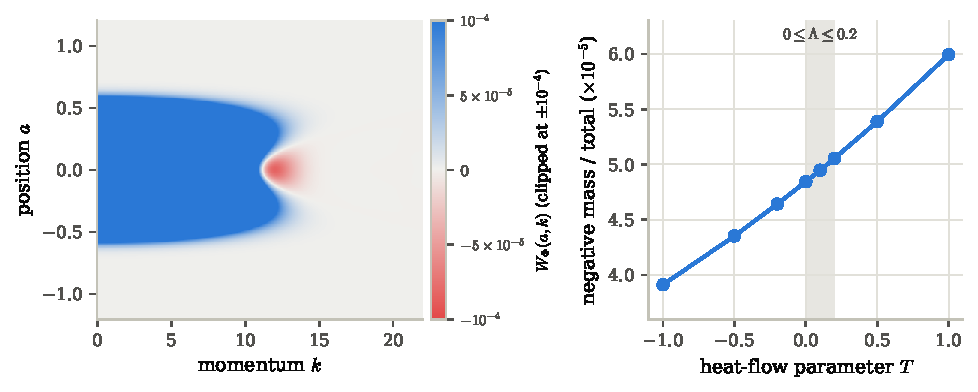
\includegraphics[width=\textwidth]{fig_negativity.pdf}
\caption{Left: $W_\Phi(a,k)$ (unnormalised, clipped at $\pm10^{-4}$) on $|a|\le1.2$, $0\le k\le22$; the negative lobe (red) lies on and near the axis $a=0$ for $11.2<k<15.8$. Right: negative Wigner mass as a fraction of the total at the eight values of $T$ of \cref{tab:neg}, along the heat flow $\Phi\mapsto e^{T\tau^2/4}\Phi$; the band marks the interval $0\le\Lambda\le0.2$ that contains the de Bruijn--Newman constant.}
\label{fig:neg}
\end{figure}

\section{The heat flow is Gaussian filtering}\label{sec:flow}
Let $\Phi_T(\tau)=e^{T\tau^2/4}\Phi(\tau)$ and $\Xi_T(z)=\int_0^\infty\Phi_T(\tau)\cos(z\tau)\dd\tau$. In the normalisation of Polymath \cite{Polymath}, $\Xi_T(z)=8H_T(2z)$ with $H_T(z)=\int_0^\infty e^{Tu^2}\Phi_{\mathrm P}(u)\cos(zu)\dd u$ the de Bruijn--Newman family (substitute $\tau=2u$; $\Phi(2u)=4\Phi_{\mathrm P}(u)$), and $\Xi_0=\Xi$. Since $\Phi_T>0$, $\Xi_T(0)>0$; and since $|\cos(z\tau)|\le e^{|y|\tau}$ and $\Phi_T(\tau)\le C_Te^{5\tau+|T|\tau^2/4-\pi e^{2\tau}}$ for $\tau\ge0$, $|\Xi_T(x+iy)|\le\exp(O(|y|\log|y|))$, so $\Xi_T$ is entire of order at most one. For $T<0$ the map $\Phi\mapsto\Phi_T$ is multiplication by a Gaussian, an operator $e^{T\hat a^2/4}$ of operator norm one: implemented as a measurement outcome it is a heralded filter, succeeding with probability $\|\Phi_T\|^2/\|\Phi\|^2$. For $T>0$ it is an amplification, not a physical operation.

\begin{proposition}\label{prop:flow}
$\partial_T\Xi_T=-\frac14\Xi_T''$, and with $\mathcal E_T(x,y)=|\Xi_T(x+iy)|^2$ and $J_T=2\partial_y\mathcal E_T$:
\[
\partial_T\mathcal E_T=\tfrac18\bigl(\partial_y^2-\partial_x^2\bigr)\mathcal E_T,\qquad\partial_TJ_T=\tfrac18\bigl(\partial_y^2-\partial_x^2\bigr)J_T .
\]
This is forward diffusion in $y$ and backward diffusion in $x$; it has no maximum principle, and positivity of $J_T$ at one $T$ cannot be transported to smaller $T$ by comparison.
\end{proposition}
\begin{proof}
Differentiating under the integral gives $\partial_T\Xi_T=\frac14\int\tau^2\Phi_T\cos(z\tau)\dd\tau=-\frac14\Xi_T''$. For analytic $F$, $\partial_x^2|F|^2=2\Re(\bar FF'')+2|F'|^2$ and $\partial_y^2|F|^2=-2\Re(\bar FF'')+2|F'|^2$, so $\partial_T|\Xi_T|^2=-\frac12\Re(\bar\Xi_T\Xi_T'')=\frac18(\partial_y^2-\partial_x^2)|\Xi_T|^2$. The operator commutes with $\partial_y$, which gives the equation for $J_T$.
\end{proof}
\noindent With $\Xi_T$ computed by quadrature, the central difference in $T$ (step $10^{-4}$) and $\frac18(\mathcal E_{yy}-\mathcal E_{xx})$ from central second differences (step $10^{-3}$) agree to $3\times10^{-8}$, $6\times10^{-9}$, $1.2\times10^{-7}$ relative at $(x,y,T)=(3,0.4,0.1),(8,0.2,-0.3),(12,0.5,0.2)$, the level of the finite-difference error.

The de Bruijn--Newman constant $\Lambda$ is defined by: $H_T$ (equivalently $\Xi_T$) has only real zeros if and only if $T\ge\Lambda$ \cite{deBruijn,Newman}. The argument of \cref{thm:witness}(iii) uses only that $\Xi_T$ is even, real on $\R$, entire of order at most one and nonzero at $0$, which holds for every $T$. Hence:

\begin{corollary}\label{cor:boundary}
For each $T$, the family detects $\varphi_T=\Phi_T/\|\Phi_T\|$ if and only if $T<\Lambda$. Since $\Lambda\ge0$ \cite{RT}, every filter $e^{T\hat a^2/4}$ with $T<0$ produces a detected state; since $\Lambda\le0.2$ \cite[Cor.~2]{PT}, no state with $T\ge0.2$ is detected. RH is the statement $\Lambda=0$: the unfiltered kernel lies exactly on the boundary between detected and undetected states.
\end{corollary}

\begin{table}[t]\centering\small
\begin{tabular}{@{}lcccccccc@{}}\toprule
$T$ & $-1$ & $-0.5$ & $-0.2$ & $0$ & $0.1$ & $0.2$ & $0.5$ & $1$\\\midrule
negative mass / total ($\times10^{-5}$) & $3.912$ & $4.353$ & $4.642$ & $4.844$ & $4.948$ & $5.055$ & $5.388$ & $5.993$\\\bottomrule
\end{tabular}
\caption{Negative Wigner mass of the filtered state $\varphi_T$ as a fraction of the total, on the grid of \cref{sec:state} with $\Phi_T$ in place of $\Phi$; halving both steps changes each entry by less than $2\times10^{-5}$ relative.}\label{tab:neg}
\end{table}

\paragraph{The amount of negativity is not what is detected.} At the eight sampled values in \cref{tab:neg} the negative fraction increases with $T$, with no visible feature in $[0,0.2]$ (\cref{fig:neg}, right). For $T<0$ this is generic rather than special to $\Phi$: since $(a+\frac s2)^2+(a-\frac s2)^2=2a^2+\frac{s^2}2$, the Wigner function of $e^{T\hat a^2/4}\psi$ is $e^{Ta^2/2}$ times the Fourier transform in $s$ of $e^{Ts^2/8}\psi(a+\frac s2)\psi(a-\frac s2)$, i.e.\ $e^{Ta^2/2}$ times the convolution of $W_\psi(a,\cdot)$ with a Gaussian of variance $|T|/4$ in momentum, which smooths negative lobes for any state. The filtered states with $T<0$ carry less negativity and yet are detected; those with $T\ge0.2$ carry more and are not. Detection and amount of negativity are not monotonically related, in line with \cref{thm:witness}(i): the family responds to the analytic structure of $\tilde\varphi$, not to a scalar measure of non-classicality.

\section{Two copies and a beamsplitter}\label{sec:beam}
The substitution $p=u+v$, $q=u-v$ that defines $Q$ from $\Phi(u)\Phi(v)$ is, up to rescaling of both outputs, a balanced beamsplitter acting on two copies of the state. Under it a product of Gaussian filters stays a product, $e^{T(u^2+v^2)/4}=e^{T(p^2+q^2)/8}$: along the flow, $Q_T$ is $Q$ reweighted by $e^{Tp^2/8}$ in the sum port and, for $T<0$, smoothed by a Gaussian in the momentum conjugate to the difference port. $Q(\cdot,x)$ is thus the sum-port amplitude conditioned on a homodyne measurement of the difference port with outcome $x$; at $x=0$ it is $2(\Phi*\Phi)$ (substitute $u=\frac{p+q}2$). Iterated self-convolution drives states toward Gaussians, the mechanism exploited, with vacuum heralding in place of homodyne conditioning, in the Gaussification scheme of \cite{BESP}.

\section{Decoherence at the thirds}\label{sec:thirds}
We now turn from the kernel as an amplitude to a probe that reads a distribution. A qubit prepared in $|+\rangle$ and coupled to a bath by $\lambda\sigma_z\otimes B$ records the bath in its coherence.

\begin{lemma}[coherence is a characteristic function]\label{lem:char}
Let $\mathcal H=\lambda\sigma_z\otimes B$ and $\rho(0)=|+\rangle\langle+|\otimes\rho_B$. Then $\rho_{01}(t)=\frac12L(t)$ with $L(t)=\operatorname{Tr}(\rho_Be^{-2i\lambda tB})=\sum_bp_b\,e^{-2i\lambda tb}$, where $p_b=\operatorname{Tr}(\rho_B\Pi_b)$ and $\Pi_b$ projects onto the eigenvalue $b$ of $B$.
\end{lemma}
\begin{proof}
Since $\sigma_z|0\rangle=|0\rangle$ and $\sigma_z|1\rangle=-|1\rangle$, $e^{-i\mathcal Ht}=|0\rangle\langle0|\otimes e^{-i\lambda tB}+|1\rangle\langle1|\otimes e^{i\lambda tB}$. With $\rho(t)=e^{-i\mathcal Ht}\rho(0)e^{i\mathcal Ht}$ and $\langle0|{+}\rangle\langle{+}|1\rangle=\frac12$, this gives $\rho_{01}(t)=\langle0|\operatorname{Tr}_B\rho(t)|1\rangle=\frac12\operatorname{Tr}(e^{-i\lambda tB}\rho_Be^{-i\lambda tB})=\frac12\operatorname{Tr}(\rho_Be^{-2i\lambda tB})$ by cyclicity of the trace. Inserting $e^{-2i\lambda tB}=\sum_be^{-2i\lambda tb}\Pi_b$ gives the sum.
\end{proof}
The probe sees only the distribution of $B$. Complete decoherence, $L=0$, is destructive interference among the values of $B$.

\begin{proposition}[the thirds]\label{prop:thirds}
For $B=S_z$ on a spin-1 with $\rho_B=I/3$, \cref{lem:char} with $p_m=\frac13$ gives $L(t)=(1+2\cos2\lambda t)/3=(z^{-1}+1+z)/3$ with $z=e^{-2i\lambda t}$. $L$ has period $\pi/\lambda$ and vanishes exactly at $t=\pi/3\lambda$ and $2\pi/3\lambda$, which are $\frac13$ and $\frac23$ of the revival period. There $z$ is a primitive cube root of unity. Midway between the two zeros, $L=-\frac13$.
\end{proposition}
\begin{proof}
$L=0$ exactly when $\cos2\lambda t=-\frac12$, that is $2\lambda t\equiv2\pi/3$ or $4\pi/3\pmod{2\pi}$; then $z=e^{\mp2\pi i/3}$ and $1+z+z^2=0$. At $t=\pi/2\lambda$, $\cos\pi=-1$ gives $L=-\frac13$.
\end{proof}
\emph{Direct evolution.} Forming $U=\exp(-i\mathcal Ht)$ as a $6\times6$ matrix exponential on $\C^2\otimes\C^3$, evolving $\rho(t)=U\rho(0)U^{-1}$ and tracing out the bath, for $\lambda\in\{1,0.37\}$ at $2001$ equally spaced times over two periods, reproduces the closed form to $5.6\times10^{-16}$. The zeros of the closed form, located by bracketing root-finding, lie at $\lambda t/\pi=\frac13,\frac23$ to $1.1\times10^{-16}$, the simulated $|L|$ there is at most $3.9\times10^{-16}$, and the revival $L(\pi/\lambda)=1$ holds to $2.2\times10^{-16}$ (\cref{fig:main}a).

\section{The spin-1 as a merged pair}\label{sec:merge}
\begin{proposition}[merged pair]\label{prop:merge}
Let $\mu_1,\mu_2\in\{\pm\frac12\}$ carry weight $e^{4g\mu_1\mu_2}$. Then $S=\mu_1+\mu_2$ has weights $e^g,2e^{-g},e^g$ at $S=-1,0,1$ (aligned spins have $4\mu_1\mu_2=1$, opposed ones $-1$). These are equal, each $\sqrt2$, exactly at $g=\frac12\ln2$. A probe coupled by $\lambda\sigma_z\otimes(\mu_1^z+\mu_2^z)$ to the Gibbs state $\propto e^{4g\mu_1^z\mu_2^z}$ with $g=\frac12\ln2$ therefore has, by \cref{lem:char}, the coherence of \cref{prop:thirds}. The unmerged pair, $g=0$, gives $L=\cos^2\lambda t$, with a double zero at half the period.
\end{proposition}
\begin{proof}
$S=\pm1$ arises from one aligned configuration each, $S=0$ from the two opposed ones. The weights are equal when $e^g=2e^{-g}$, i.e.\ $e^{2g}=2$, and then each is $e^g=\sqrt2$. At $g=0$ the weights $1,2,1$ give $L=(e^{2i\lambda t}+2+e^{-2i\lambda t})/4=(1+\cos2\lambda t)/2=\cos^2\lambda t$, which vanishes to second order at $\lambda t=\pi/2$.
\end{proof}
\paragraph{The quantum merge and the fourth state.} As a representation, $\frac12\otimes\frac12=1\oplus0$. The triplet $\{|{\uparrow\uparrow}\rangle,(|{\uparrow\downarrow}\rangle+|{\downarrow\uparrow}\rangle)/\sqrt2,|{\downarrow\downarrow}\rangle\}$ is the triad. The singlet, also with $m=0$, is a fourth state; adding it with equal weight turns the thirds into $1{:}2{:}1$ and $\cos^2\lambda t$. Under isotropic exchange $-g\,\mathbf S_1\!\cdot\!\mathbf S_2$ at inverse temperature $\beta$, since $\mathbf S_1\!\cdot\!\mathbf S_2=\frac12(\mathbf S^2-\frac32)$ equals $\frac14$ on the triplet and $-\frac34$ on the singlet, the triplet levels have weight $e^{\beta g/4}$ and the singlet $e^{-3\beta g/4}$. Hence $P(0)/P(\pm1)=(e^{\beta g/4}+e^{-3\beta g/4})/e^{\beta g/4}=1+e^{-\beta g}$, and this quantum merge reaches the thirds only as the fourth state is frozen out ($\beta g\to\infty$). The Ising merge reaches them exactly, at the finite coupling $\frac12\ln2$. Diagonalising the Gibbs state at $\beta g=1$ gives $P(0)/P(\pm1)=1.367879441171=1+e^{-1}$.

\emph{Direct evolution.} At $g=\frac12\ln2=0.346573590280$ the summed weights are all $1.414213562373$ (relative spread $1.6\times10^{-16}$). The matrix-exponential evolution of \cref{sec:thirds}, with the two-spin Ising Gibbs state as bath, gives the thirds to $3.3\times10^{-16}$; numerical diagonalisation of $\mathbf S^2$ gives eigenvalues $(2,2,2,0)$; the maximally mixed triplet gives the thirds to $5.6\times10^{-16}$ and the maximally mixed four-state space $\cos^2\lambda t$ to $3.3\times10^{-16}$.

\section{Lee--Yang zeros as complete-decoherence times}\label{sec:ly}
Take an open chain of $N$ uniform three-state spins $S_i\in\{-1,0,1\}$ in the Gibbs state $\propto\exp(K\sum S_iS_{i+1})$ at zero field, and couple the probe by $\lambda\sigma_z\otimes\sum S_i^z$. By \cref{lem:char}, with $p_b$ the Gibbs probability that $\sum S_i=b$,
\[
L(t)=\frac{Z(e^{-2i\lambda t})}{Z(1)},\qquad Z(z)=\sum_{\{S\}}e^{K\sum S_iS_{i+1}}\,z^{\sum S_i}=\sum_{m=-N}^{N}c_mz^m,
\]
the Wei--Liu identity \cite{WeiLiu} for this bath; $c_m>0$ is the total weight of the configurations with $\sum S_i=m$, and $z$ is the fugacity. Spin reversal gives $c_{-m}=c_m$, so $Z(z)=Z(1/z)$ with real coefficients, the zeros come in sets $\{z,\bar z,1/z,1/\bar z\}$, and for real $t$, with $\theta=2\lambda t$,
\[
L=\frac{c_0+2\sum_{m=1}^{N}c_m\cos m\theta}{Z(1)}
\]
is real. A zero with $|z|=1$ is a real time of complete decoherence; a zero off the circle is a complex time, where $L$ does not vanish.

\begin{theorem}[merged-pair Lee--Yang]\label{thm:ly}
If $K\ge0$, all $2N$ zeros of $z^NZ(z)$ lie on $|z|=1$. Equivalently, $L$ continued to complex $t$ vanishes only at real $t$, at $2N$ times per period counted with multiplicity, and every local minimum of $|L|$ at real times is a zero. At $K=0$, $z^NZ=(1+z+z^2)^N$, so $L=\bigl((1+2\cos2\lambda t)/3\bigr)^N$ has $N$-fold zeros exactly at the thirds.
\end{theorem}
\begin{proof}
By \cref{prop:merge}, the uniform measure on $\{-1,0,1\}$ is, up to the factor $\sqrt2$, the law of $\mu_{i1}+\mu_{i2}$ under the weight $e^{2\ln2\,\mu_{i1}\mu_{i2}}$. Substitute this for every $S_i$: for each configuration $\{S\}$ the sum of $\prod_ie^{2\ln2\,\mu_{i1}\mu_{i2}}$ over the $\mu$'s with $\mu_{i1}+\mu_{i2}=S_i$ is $(\sqrt2)^N$. Then $KS_iS_{i+1}=K\sum_{j,j'}\mu_{ij}\mu_{i+1,j'}$ and $z^{S_i}=z^{\mu_{i1}}z^{\mu_{i2}}$, so $2^{N/2}Z$ is the partition function of $2N$ spin-$\frac12$'s with nonnegative pair couplings ($\frac12\ln2$ within a pair, $K/4$ between neighbouring pairs, in the variables $\sigma=2\mu=\pm1$) in a uniform field $z$. The Lee--Yang circle theorem \cite{LeeYang} puts every zero of $z^NZ(z)$ on $|z|=1$. This polynomial has degree $2N$ and constant term $c_{-N}=e^{K(N-1)}\ne0$, so it has exactly $2N$ zeros, each giving one real $t$ modulo $\pi/\lambda$; $|z|=1$ is the same as $t$ real. The case $K=0$ is a product of copies of \cref{prop:thirds}.

For the minima: $L$ is a trigonometric polynomial of degree $N$ in $\theta$ with leading coefficient $2c_N/Z(1)\ne0$, so $e^{iN\theta}L'(\theta)$ is a nonzero polynomial of degree at most $2N$ in $e^{i\theta}$ and $L'$ has at most $2N$ zeros per period, counted with multiplicity. Let $L$ have distinct zeros $\theta_1<\dots<\theta_r$ in one period with multiplicities $m_j$, $\sum m_j=2N$. Each $\theta_j$ is a zero of $L'$ of multiplicity $m_j-1$, and by Rolle's theorem each of the $r$ gaps between cyclically consecutive zeros contains a zero of $L'$. This already gives $\sum(m_j-1)+r=2N$ zeros of $L'$, so each gap contains exactly one, which is simple. On a gap $|L|$ rises from $0$ and returns to $0$, so its only critical point there is a maximum. At a real $t$ with $L\ne0$, a local minimum of $|L|$ would need $L'=0$; hence every local minimum of $|L|$ is a zero.
\end{proof}
The companion paper \cite{SMath} proves the circle statement for three-state spins with arbitrary nonnegative couplings $K_{ij}$ by the same substitution.

\paragraph{Example: two triads.} For $N=2$ the nine configurations give $c_{\pm2}=e^K$, $c_{\pm1}=2$, $c_0=1+2e^{-K}$ and $Z(1)=2e^K+5+2e^{-K}$. With $v=\cos\theta$ and $\cos2\theta=2v^2-1$,
\[
L=\frac{4e^Kv^2+4v+1+2e^{-K}-2e^K}{2e^K+5+2e^{-K}} .
\]
The quadratic in $v$ has discriminant $16(2e^K+1)(e^K-1)$, which is nonnegative exactly when $K\ge0$. At $K=1$ its roots $v=\bigl(-1\pm\sqrt{(2e+1)(e-1)}\bigr)/2e=0.42778$ and $-0.79566$ give the four real zeros $\theta/2\pi=\lambda t/\pi=0.179649$, $0.396437$, $0.603563$, $0.820351$. At $K=-1$ the roots are complex, the vertex $v=-e/2$ lies outside $[-1,1]$, and $|L|$ is smallest at $v=-1$ ($\lambda t/\pi=\frac12$), where $L=(2e^K+2e^{-K}-3)/(2e^K+5+2e^{-K})=0.2839$.

\paragraph{Chains with $K>0$.} The coefficients $c_m$ come from exhaustive enumeration of the $3^N$ configurations; at $K=0$ they equal those of $(1+z+z^2)^N$ exactly (e.g.\ $1,3,6,7,6,3,1$ at $N=3$). For $N=2,\dots,6$ and $K\in\{0.1,0.5,1,2\}$ the roots of $z^NZ(z)$, computed as the eigenvalues of its companion matrix, all satisfy $||z|-1|\le8.2\times10^{-14}$, and the smallest distance between two roots is $0.168$, so the $2N$ decoherence times are distinct. On one period, $\theta\in[0,2\pi)$ sampled at $2\times10^5$ equally spaced points, $L$ has exactly $2N$ sign changes and $|L|$ exactly $2N$ discrete local minima; the zeros, refined by bracketing root-finding (Brent's method, tolerance $10^{-14}$), match the arguments $-\arg z_j$ of the roots to $1.9\times10^{-13}$, and $|L|\le4.0\times10^{-15}$ at every refined zero, so each of the $2N$ discrete minima is a complete decoherence, as \cref{thm:ly} requires. Full unitary evolution on $\C^2\otimes\C^{3^N}$ for $N=2,3$ and $K=\pm1$ agrees with $Z(e^{-2i\lambda t})/Z(1)$ to $3.3\times10^{-16}$.

\begin{table}[t]\centering\small
\begin{tabular}{@{}cccccc@{}}\toprule
$N$ & on circle & $\max|z|$ & $\min_j|L(t_j)|$ & positive minima of $|L|$ & real zeros, $\lambda t/\pi$\\\midrule
2 & 0 of 4 & 3.9719 & 0.3344 & 0.2839 & none\\
3 & 2 of 6 & 8.7699 & 0.06584 & none & 0.33353, 0.66647\\
4 & 0 of 8 & 11.4872 & 0.1387 & 0.1212 & none\\
5 & 2 of 10 & 13.0181 & 0.01504 & none & 0.34207, 0.65793\\
6 & 0 of 12 & 13.9393 & 0.05831 & 0.05311 (twice) & none\\\bottomrule
\end{tabular}
\caption{The antiferromagnetic chain, $K=-1$. Off-circle roots come in mirrored pairs $z,1/\bar z$; $t_j$ is the time at which $e^{-2i\lambda t_j}$ points towards an off-circle root; positive minima are strictly positive local minima of $|L|$.}\label{tab:afm}
\end{table}

\paragraph{The antiferromagnet.} For $K=-1$ the merged-pair argument does not apply and its conclusion fails (\cref{tab:afm}, \cref{fig:main}b), as the example already shows for $N=2$. For every $N=2,\dots,6$ roots leave the circle, to $\max|z|$ between $3.9719$ and $13.9393$, and the number of sign changes of $L$ per period equals the number of roots on the circle. For even $N$ no zero is on the circle and the probe never fully decoheres ($|L|\ge0.2839$, $0.1212$, $0.05311$ for $N=2,4,6$); for odd $N$ one pair stays on the circle, near the thirds. At the time $t_j$ of every off-circle root $|L(t_j)|\ge0.01504$. Every local minimum of $|L|$ is either a zero on the circle or at least $0.05311$: no dip of $|L|$ lies between zero and $0.05311$. The ferromagnetic merge makes every dip a complete decoherence; the antiferromagnet leaves dips that stop short of zero.

\begin{figure}[t]\centering
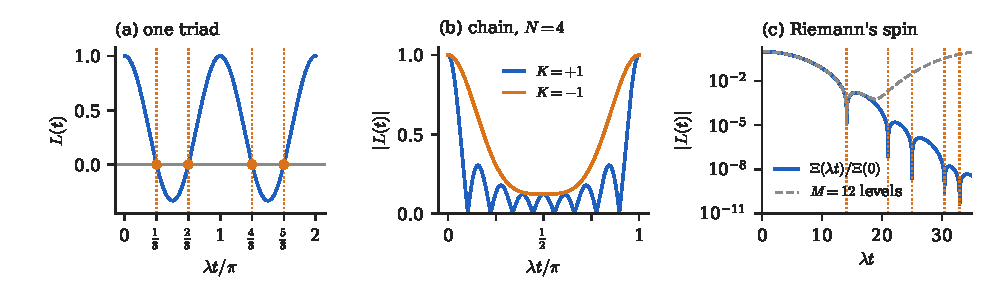
\includegraphics[width=\textwidth]{fig_decoherence.pdf}
\caption{(a) One triad: complete decoherence at $\frac13$ and $\frac23$ of each revival period. (b) $|L|$ for a chain of $N=4$ triads. With $K=+1$ it reaches zero eight times per period. With $K=-1$ no zero lies on the circle and $|L|\ge0.1212$. (c) Riemann's spin: $|L|=|\Xi(\lambda t)/\Xi(0)|$ vanishes at $\gamma_1,\dots,\gamma_5$ (dotted). Dashed: a bath of $M=12$ classical levels; it reproduces $\gamma_1$ to $3.2\times10^{-4}$, then shows a positive dip ($5.83\times10^{-4}$ at $\lambda t=18.845$) from a complex zero at $19.0235+1.6456i$.}\label{fig:main}
\end{figure}

\section{Riemann's spin}\label{sec:riemann}
The kernel of \cref{sec:state} is positive and even, and $\int_\R\Phi=2\Xi(0)$, so $P_\Phi=\Phi/(2\Xi(0))$ is a probability density. A probe whose spin $\sigma_z/2$ couples to a classical field $\tau$ with this law, $\mathcal H=\lambda(\sigma_z/2)\tau$, is \cref{lem:char} with $B=\tau/2$ acting by multiplication, so
\[
L(t)=\int_\R P_\Phi(\tau)e^{-i\lambda t\tau}\dd\tau=\frac{\Xi(\lambda t)}{\Xi(0)}=\frac{\tilde\varphi(\lambda t)}{\tilde\varphi(0)},
\]
the sign of the exponent being immaterial because $P_\Phi$ is even; the last form is the normalised momentum wave function of the Riemann state, since $\tilde\varphi=(2/\pi)^{1/2}\,\Xi/\|\Phi\|$. The same function thus serves as the amplitude of $\varphi$ and as the law of the bath.

\begin{proposition}[the Riemann probe]\label{prop:riemann}
\begin{enumerate}
\item $L(t)=0$ at real $t$ exactly when $\frac12\pm i\lambda t$ is a zero of $\zeta$ on the critical line. In particular $L$ vanishes at $\lambda t=\gamma_n$.
\item RH holds if and only if the coherence $L$, continued to complex time, vanishes only at real times.
\item If RH holds, every local minimum of $|L|$ at real times is a zero, so the probe never shows a partial dip. Equivalently, a strictly positive local minimum of $|\Xi|$ on $\R$ would contradict RH.
\end{enumerate}
\end{proposition}
\begin{proof}
Parts (1) and (2) hold because $\Xi(z)=\xi(\frac12+iz)$, the zeros of $\xi$ are the nontrivial zeros of $\zeta$, and $\lambda>0$ is real. For (3), use the product \cref{eq:hadamard}. Under RH every $z_n$ is real, and on each interval of $\R$ free of zeros, including $(-z_1,z_1)$,
\[
\frac{\dd}{\dd x}\frac{\Xi'(x)}{\Xi(x)}=-\sum_n\Bigl[\frac1{(x-z_n)^2}+\frac1{(x+z_n)^2}\Bigr]<0 ,
\]
the series converging uniformly on compact subsets of the interval. So between consecutive zeros $\Xi'/\Xi$ falls strictly from $+\infty$ to $-\infty$ and vanishes exactly once, at a maximum of $|\Xi|$. Since a local minimum of $|\Xi|$ at a point where $\Xi\ne0$ needs $\Xi'=0$, every local minimum is a zero.
\end{proof}
This is \cref{sec:ly} for one continuous spin. The real time axis is the Lee--Yang circle, since the single-spin partition function in a field $h$ is $Z_1(h)=\frac12\int_\R\Phi(\tau)e^{h\tau}\dd\tau=\Xi(-ih)$, and RH says that Riemann's spin behaves like the ferromagnet of \cref{thm:ly}. Along the heat flow the three readings of this paper become one condition:

\begin{corollary}\label{cor:three}
For real $T$ let $\varphi_T=\Phi_T/\|\Phi_T\|$ and let $L_T(t)$ be the coherence of a probe dephased, as above, by a field with law $\Phi_T/\int\Phi_T$. The following are equivalent: (a) $T\ge\Lambda$; (b) the family $\hat O_{x,y}$ does not detect $\varphi_T$; (c) $L_T$, continued to complex time, vanishes only at real times. For $T\ge\Lambda$ every local minimum of $|L_T|$ at real times is a zero. In particular every Gaussian-filtered bath with $T<0$ has complete-decoherence times off the real axis, and every bath with $T\ge0.2$ has none.
\end{corollary}
\begin{proof}
$\Phi_T$ is positive, even and integrable, so as above $L_T(t)=\Xi_T(\lambda t)/\Xi_T(0)$, and (c) says that $\Xi_T$ has only real zeros, which is (a) by the definition of $\Lambda$. (a)$\Leftrightarrow$(b) is \cref{cor:boundary}. The proof of \cref{prop:riemann}(3) uses only that the function is even, real on $\R$, entire of order at most one, nonzero at $0$ and has only real zeros, all of which hold for $\Xi_T$ when $T\ge\Lambda$. The last sentence follows from $0\le\Lambda\le0.2$ \cite{RT,PT}.
\end{proof}

\paragraph{The Riemann coherence.} We summed the series for $\Phi$ at $|\tau|$ to $n=12$ (at $\tau=0$ the first omitted term is below $e^{-516}$, and later terms are smaller still) and evaluated $\Xi(t)=\frac12\int_\R\Phi(\tau)\cos(t\tau)\dd\tau$ by the trapezoid rule on $[-3,3]$ with step $10^{-3}$. Beyond $|\tau|=3$, $\Phi<e^{-1200}$; the integrand is analytic in the strip $|\Im\tau|<\pi/4$ and decays faster than exponentially, so the trapezoid rule is accurate to rounding level, and indeed halving the step changes $\Xi$ on $[0,35]$ by at most $1.1\times10^{-16}$. This gives $\Xi(0)=0.4971207781883141$, equal to $\xi(\frac12)=-\zeta(\frac12)\Gamma(\frac14)\pi^{-1/4}/8$ (the definition of $\xi$ at $s=\frac12$, with the values of \cref{sec:data}) to $5.6\times10^{-17}$. Evenness holds numerically as well: the series summed directly at $-\tau$ (to $n=60$) agrees with its value at $\tau$ to relative $1.0\times10^{-14}$ on $[0,\frac12]$, and $\Phi>0$ on $[0,2.5]$. On a grid of step $0.01$, $L$ has exactly five sign changes in $(0,35)$; refined by bracketing root-finding they lie at $14.1347251417$, $21.0220396388$, $25.0108575801$, $30.4248761260$ and $32.9350615890$. These lie within $1.0\times10^{-9}$ of the ordinates tabulated to nine decimals \cite{Odlyzko} (\cref{sec:data}); the largest deviation is at $\gamma_5$, where $|L'|=8.2\times10^{-9}$, so that a rounding error of order $10^{-17}$ in $L$ moves the computed zero by order $10^{-9}$. The five discrete local minima of $|L|$ on the same grid in $(0.5,35)$ are exactly these zeros, as \cref{prop:riemann}(3) requires under RH. Between consecutive zeros the maximum of $|L|$, found by bounded one-dimensional maximisation, is $1.6\times10^{-3}$, $1.6\times10^{-5}$, $1.3\times10^{-6}$ and $1.6\times10^{-8}$ (\cref{fig:main}c).

\paragraph{A probe coupled to $M$ classical levels.} We discretise $P_\Phi$ by its $M$-point Gauss rule. The measure $P_\Phi(\tau)\dd\tau$ is replaced by the discrete measure of the trapezoid rule with step $5\times10^{-4}$ on $[-3,3]$; the Lanczos process with full reorthogonalisation, applied to multiplication by $\tau$ with starting vector $\sqrt{P_\Phi}$, produces the $M\times M$ Jacobi matrix of the orthonormal polynomials of this measure, whose eigenvalues are the nodes $\tau_j$ and whose squared normalised first eigenvector components are the weights $w_j$ (Golub--Welsch \cite{GolubWelsch}). This gives levels $\tau_j$ with populations $w_j>0$ (for all $M\in\{4,8,12,16,24,32,48,64\}$) and coherence $L_M(t)=\sum_jw_j\cos(\lambda t\tau_j)$, whose real zeros we locate on a grid of step $0.005$ and refine by bracketing. The errors of the nearest real zeros to $\gamma_1,\gamma_2,\gamma_3$, measured against the nine-decimal ordinates (whose rounding contributes up to $2.7\times10^{-10}$), are $1.8\times10^{-8}$, $0.113$ and none (no real zero nearby) at $M=16$; $2.7\times10^{-10}$, $3.4\times10^{-9}$, $7.2\times10^{-5}$ at $M=24$; and $2.7\times10^{-10}$, $2.5\times10^{-10}$, $7.1\times10^{-10}$ at $M=64$. Over every $M\le40$, $\gamma_1,\dots,\gamma_5$ first appear within $10^{-6}$ at $M=15,22,27,33,36$. The finite bath shows the mechanism of \cref{sec:ly}: its first zeros are real and accurate, their range grows with $M$, and beyond it zeros are displaced and some leave the real axis, where the probe shows a positive dip instead. For $M=12$, Newton's method for the entire function $L_M$, started from a grid of complex points, finds a zero at $19.0235+1.6456i$, and the real-time coherence has a dip of depth $5.83\times10^{-4}$ at $\lambda t=18.845$.

\section{An experimental proposal}\label{sec:exp}
\emph{One triad.} As in Peng et al.\ \cite{Peng}, one records the coherence of a probe nucleus against time and reads off its zeros. A spin-$\frac12$ probe such as $^{13}$C, scalar-coupled with coupling constant $\mathcal J$ (in Hz) to one deuteron (spin 1), has $\mathcal H=2\pi\mathcal JI_z^XS_z^D=\pi\mathcal J\sigma_zS_z$ in the weak-coupling limit, so $\lambda=\pi\mathcal J$. At room temperature the deuteron is effectively maximally mixed. \Cref{prop:thirds} then gives the on-resonance envelope $(1+2\cos2\pi\mathcal Jt)/3$, with zeros at $t=1/3\mathcal J$ and $2/3\mathcal J$ and a revival at $1/\mathcal J$. In frequency this is the familiar $1{:}1{:}1$ triplet of a carbon bonded to deuterium; a carbon with two equivalent protons is the unmerged pair ($1{:}2{:}1$, a double zero at $1/2\mathcal J$). Quadrupolar relaxation of the deuteron (much faster for $^{14}$N) collapses the multiplet unless its relaxation time is long compared with $1/\mathcal J$.

\emph{Chains.} $N$ equivalent deuterons realise $K=0$. For a CD$_3$ group, \cref{thm:ly} gives $L=((1+2\cos2\pi\mathcal Jt)/3)^3$, with threefold zeros at the thirds and multiplet intensities $1{:}3{:}6{:}7{:}6{:}3{:}1$. For $K\ne0$ the bath needs the Gibbs distribution of $\sum S_i$. By \cref{lem:char}, $L$ depends linearly on these populations alone, so the Gibbs weights can be imposed on prepared populations or applied to separately recorded signals. For $N=2$ the experiment is sharp (the example in \cref{sec:ly}, with $\lambda t/\pi=\mathcal Jt$): at $K=1$ complete decoherence at $\mathcal Jt=0.179649$, $0.396437$, $0.603563$, $0.820351$; at $K=-1$ none, with $|L|\ge0.2839$.

\emph{The discretised Riemann bath.} Repeat a Ramsey sequence with the probe detuned by the angular frequency $\lambda\tau_j$ in the $j$th repetition and sum the signals with weights $w_j$. The summed signal is the coherence $L_M$ of \cref{sec:riemann}. With $M=15$ levels its first zero lies within $10^{-6}$ of $\gamma_1$; with $M=64$ its first three zeros reproduce $\gamma_1,\gamma_2,\gamma_3$ to $7.1\times10^{-10}$. Between $\gamma_1$ and $\gamma_2$ the coherence peaks at only $1.6\times10^{-3}$, so the signal must be accurate well below that level, and each later zero needs one to two further decades of dynamic range. A positive dip in the recorded signal, as at $\lambda t=18.845$ for $M=12$, marks a zero of $L_M$ that has left the real axis.

\section{Proof of the tail-positivity theorem}\label{sec:tail}
This section gives in full, in the present notation, the argument of the companion paper \cite{SMath} on which \cref{prop:confine} rests. Write $K_{ix}(z)=\int_0^\infty e^{-z\cosh w}\cos(xw)\dd w$ ($z>0$) for the Macdonald function of imaginary order, which is real, and $d(N)$ for the number of divisors of $N$.

\begin{lemma}[Macdonald expansion]\label{lem:macdonald}
For all real $p,x$, with $\omega_N=2\pi Ne^p$,
\[
Q(p,x)=8e^{p/2}\sum_{N\ge1}\tau_x(N)\,\mathcal K_x(\omega_N),\qquad\tau_x(N)=\sum_{mn=N}\cos\Bigl(x\log\frac mn\Bigr),
\]
with $\mathcal K_x(z)=(z^4+9z^2)K_{ix}(z)+6z^3K'_{ix}(z)$.
\end{lemma}
\begin{proof}
Insert the theta series for $\Phi(u)$ and $\Phi(v)$, $u=\frac{p+q}2$, $v=\frac{p-q}2$, valid for all real arguments (\cref{sec:state}). For fixed $p$ the double series of absolute values is $O(e^{|u|/2})$ in $u$, $O(e^{|v|/2})$ in $v$ and doubly-exponentially small in whichever of $u,v$ is positive, hence dominated by an integrable function of $q$, and may be integrated term by term. For the term $(m,n)$ the exponent is $-\pi(m^2e^{2u}+n^2e^{2v})=-\pi e^p(m^2e^q+n^2e^{-q})=-z\cosh(q+\kappa)$ with $z=2\pi mne^p$, $\kappa=\log\frac mn$, and the prefactor is $16$ times
\[
4\pi^4m^4n^4e^{9p/2}-6\pi^3m^4n^2e^{7p/2}e^{q}-6\pi^3m^2n^4e^{7p/2}e^{-q}+9\pi^2m^2n^2e^{5p/2}.
\]
Put $w=q+\kappa$ and use $\int_\R e^{-z\cosh w}e^{\nu w}\dd w=2K_\nu(z)$ for complex $\nu$, with $K_{-\nu}=K_\nu$ \cite[\S10.32]{DLMF}. Then $\int e^{-z\cosh(q+\kappa)}\cos(xq)\dd q=2\cos(x\kappa)K_{ix}(z)$ and $\int e^{-z\cosh(q+\kappa)}e^{\pm q}\cos(xq)\dd q=2e^{\mp \kappa}\Re[e^{-ix\kappa}K_{1\pm ix}(z)]$. The factors $e^{\mp \kappa}=(n/m)^{\pm1}$ turn both middle coefficients into $(mn)^3$, and $K_{1-ix}(z)=\overline{K_{1+ix}(z)}$ for $z>0$, so the middle terms combine to $-16\cdot6\pi^3(mn)^3e^{7p/2}\cdot4\cos(x\kappa)\Re K_{1+ix}(z)$, where $\Re K_{1+ix}(z)=\int_0^\infty e^{-z\cosh w}\cosh w\cos(xw)\dd w=-K'_{ix}(z)$. Substituting $mn=ze^{-p}/2\pi$, the term $(m,n)$ equals $8e^{p/2}\cos(x\log\frac mn)\,\mathcal K_x(z)$; summing over $mn=N$ gives $\tau_x(N)$.
\end{proof}

\begin{lemma}[Riccati bounds]\label{lem:riccati}
Let $a_x=\sqrt{x^2+\frac14}$, $\eta(z)=\sqrt z\,K_{ix}(z)$ and $c(z)=1-a_x^2/z^2$. For $z\ge a_x$: $K_{ix}(z)>0$, $K'_{ix}(z)<0$, $r:=-\eta'/\eta$ satisfies $\sqrt{c(z)}\le r(z)\le1$, and $0<-K'_{ix}(z)/K_{ix}(z)\le1+\frac1{2z}$.
\end{lemma}
\begin{proof}
$K_{ix}$ solves the modified Bessel equation $z^2w''+zw'-(z^2-x^2)w=0$ \cite[\S10.25]{DLMF}, and $w=z^{-1/2}\eta$ turns it into $\eta''=c\,\eta$. As $z\to\infty$, $K_{ix}(z)=\sqrt{\pi/2z}\,e^{-z}(1+O(1/z))$ \cite[\S10.40]{DLMF}, so $\eta\to0^+$. On $[a_x,\infty)$, $c\ge0$. If $\eta$ vanished at some $z_*\ge a_x$, take the largest such zero; on $(z_*,\infty)$, $\eta>0$ and $\eta''=c\eta\ge0$, so $\eta$ is convex there with $\eta(z_*)=0$, hence eventually increasing, contradicting $\eta\to0$. So $\eta>0$ on $[a_x,\infty)$, $\eta$ is convex there, and $\eta\to0$ forces $\eta'<0$; then $K_{ix}=z^{-1/2}\eta>0$ and $K'_{ix}=z^{-1/2}(\eta'-\eta/2z)<0$. The function $r$ is positive and finite and satisfies $r'=r^2-c$. If $r(z_*)>1$, then $r'>r^2-1$ and comparison with $\varrho'=\varrho^2-1$, $\varrho(z_*)=r(z_*)$, forces blow-up at finite $z$; if $r(z_*)<\sqrt{c(z_*)}$, then $r$ decreases while $\sqrt c$ increases, so $r'\le r(z_*)^2-c(z_*)<0$ for all $z>z_*$, driving $r$ negative. Both contradict $0<r<\infty$. Finally $-K'_{ix}/K_{ix}=r+\frac1{2z}$.
\end{proof}

\begin{theorem}[tail positivity]\label{thm:tail}
Let $\omega_1=2\pi e^{|p|}$ and $\omega_0=\max(\sqrt2\,a_x,20)$. If $\omega_1\ge \omega_0$, then
\[
Q(p,x)\ \ge\ 8\,(1-R(\omega_1))\,e^{|p|/2}\omega_1^2(\omega_1^2-6\omega_1+6)K_{ix}(\omega_1)\ >\ 0,
\]
where
\[
R(z)=\frac{\sum_{N\ge2}d(N)(N^4z^4+6N^3z^3+12N^2z^2)e^{-(N-1)z/\sqrt2}}{z^2(z^2-6z+6)},
\]
and $R(\omega_1)\le R(20)=3.74\times10^{-5}$. Since $2a_x^2=2x^2+\frac12$, the hypothesis is $2\pi e^{|p|}\ge\max(\sqrt{2x^2+\frac12},20)$.
\end{theorem}
\begin{proof}
$Q$ is even in $p$, so take $p\ge0$. Every $\omega_N=N\omega_1$ is at least $\omega_1\ge\sqrt2\,a_x\ge a_x$. By \cref{lem:riccati}, for $z\ge a_x$, $\mathcal K_x(z)\ge K_{ix}(z)[z^4+9z^2-6z^3(1+\frac1{2z})]=K_{ix}(z)\,z^2(z^2-6z+6)$ and $|\mathcal K_x(z)|\le K_{ix}(z)(z^4+6z^3+12z^2)$. On $[\omega_1,\infty)$, $c\ge\frac12$, so $(\log\eta)'=-r\le-1/\sqrt2$ and $K_{ix}(N\omega_1)\le N^{-1/2}K_{ix}(\omega_1)e^{-(N-1)\omega_1/\sqrt2}\le K_{ix}(\omega_1)e^{-(N-1)\omega_1/\sqrt2}$. With $\tau_x(1)=1$ and $|\tau_x(N)|\le d(N)$, \cref{lem:macdonald} gives $Q\ge8e^{p/2}[\mathcal K_x(\omega_1)-\sum_{N\ge2}d(N)|\mathcal K_x(N\omega_1)|]$, which is the stated bound. For $z>3+\sqrt3$ the denominator of $R$ is positive with logarithmic derivative $\frac2z+\frac{2z-6}{z^2-6z+6}\ge\frac4z$ (equivalent to $z\ge2$), while each numerator term, a polynomial of degree $4$ with positive coefficients times a decreasing exponential, has logarithmic derivative at most $\frac4z$; so every term of $R$ decreases on $[20,\infty)$ and $R(\omega_1)\le R(20)$. Summing the series, whose terms fall by factors of order $e^{-14}$, gives $R(20)=3.74\times10^{-5}$.
\end{proof}

\section{Concluding remarks}\label{sec:concl}
Riemann's kernel is a quantum state and a classical bath at once, and the two readings meet in the momentum wave function $\tilde\varphi\propto\Xi$. As a state it is Wigner-negative, with a negative lobe that is small ($4.844\times10^{-5}$ of the mass) and confined at every momentum (\cref{prop:confine}); a family of observables with nonnegative symbols detects every state whose momentum wave function has a non-real zero and no state whose momentum wave function has order at most one and only real zeros (\cref{thm:witness}). As a bath it gives a probe coherence $\Xi(\lambda t)/\Xi(0)$ whose real zeros are the Riemann ordinates. A probe qubit reads a triad as complete decoherence at $\frac13$ and $\frac23$ of its period; the triad is the merged pair; a ferromagnetic merge of triads keeps every Lee--Yang zero on the circle, so every dip reaches zero, and an antiferromagnetic one does not.

\paragraph{The remaining step.} RH is equivalent to each of the following: $J\ge0$ on the upper half-plane; nonnegativity of every even position moment of $W_\varphi$ at every momentum (\cref{thm:witness}); $\Lambda=0$, the unfiltered state lying on the detection boundary (\cref{cor:boundary}); and the probe coherence $\Xi(\lambda t)/\Xi(0)$ vanishing only at real times (\cref{prop:riemann,cor:three}). We prove $J>0$ outside $\mathcal U$ (\cref{prop:pos}) and confine the negativity of the Riemann state at momentum $x$ to $|a|<\frac12\log\frac x{2\pi}+\frac14\log2+O(x^{-2})$ (\cref{prop:confine}). The remaining step is Conjecture~\ref{conj:target}, positivity on $\mathcal U$, the step stated in \cite{SMath}: at each such momentum the positive body of $W_\varphi(\cdot,x)$ must outweigh its confined negative lobe in $\int W_\varphi(a,x)\,a\sinh(2ya)\dd a$. In the language of the merge, a sufficient route is to show that $\Phi$ lies in the Griffiths--Simon class of limits of positively merged elementary pairs, which by the Lee--Yang theorem gives RH \cite{SMath}; \cref{thm:ly} is the finite form of this statement for chains of triads, and \cref{cor:three} places the unfiltered kernel exactly at the boundary $T=\Lambda$ that this route must reach.

\paragraph{Outlook.} The NMR realisation of \cref{sec:exp} reads the thirds, the chains and the discretised Riemann bath directly from the zeros of a recorded coherence. On the analytic side the next step is Conjecture~\ref{conj:target}, the positivity of $\langle\varphi|\hat O_{x,y}|\varphi\rangle$ on $\mathcal U$, where the negative lobe is confined by \cref{prop:confine}.

\section{Data and sources}\label{sec:data}
No experimental or observational dataset is used. Every number in the paper is computed from the formulas stated in the text, by the methods stated there, except the following external inputs.
\begin{itemize}
\item \emph{Riemann's kernel.} $\Phi$ is the theta series of \cite[\S2.16]{Titchmarsh}, multiplied by $2$ to match $\Xi(z)=\int_0^\infty\Phi(\tau)\cos(z\tau)\dd\tau$; the definition of $\xi$ and the theta transformation are from \cite[Ch.~2]{Titchmarsh}, and the location of the zeros of $\xi$ in the critical strip from \cite[\S2.12 and Ch.~3]{Titchmarsh}. No zeros of $\zeta$ enter \cref{sec:state,sec:obs,sec:flow,sec:beam}: $\|\Phi\|^2=1.2790072478$, the values of $W_\Phi$ and of $J$, the negativity fractions and the sign changes on $a=0$ are computed from this series, and the same quadrature gives $\Xi(0)=\xi(\frac12)$ (\cref{sec:riemann}).
\item \emph{Riemann ordinates} (reference values only, for \cref{sec:riemann} and \cref{fig:main}c): $\gamma_1=14.134725142$, $\gamma_2=21.022039639$, $\gamma_3=25.010857580$, $\gamma_4=30.424876126$, $\gamma_5=32.935061588$, the first five entries of Odlyzko's table of the first 100 zeros of $\zeta$ (given there to over 1000 decimals) \cite{Odlyzko}, rounded to nine decimals.
\item \emph{Constants for $\xi(\frac12)$}: $\zeta(\frac12)=-1.4603545088095868$ and $\Gamma(\frac14)=3.6256099082219083$, to double precision \cite{OEIS}, giving $\xi(\frac12)=-\zeta(\frac12)\Gamma(\frac14)\pi^{-1/4}/8=0.4971207781883141$.
\item \emph{de Bruijn--Newman constant and verification height.} $0\le\Lambda$ \cite{RT} and $\Lambda\le0.2$ \cite[Cor.~2]{PT}; the earlier bounds of \cref{tab:dbn}, $\Lambda\le\frac12$ \cite{deBruijn}, $\Lambda>-\infty$ \cite{Newman} and $\Lambda\le0.22$ \cite{Polymath}; all with $\Lambda$ defined through $H_T$ in the normalisation of \cite{Polymath} ($\Xi_T(z)=8H_T(2z)$ here); all nontrivial zeros of $\zeta$ with imaginary part in $(0,3\cdot10^{12}]$ lie on the critical line \cite{PT}; $\zeta(\sigma+it)\ne0$ for $\sigma\ge1-1/(5.573412\log|t|)$, $|t|\ge2$, with the constant $5.573412$ \cite{MT} (\cref{prop:pos}).
\item \emph{Special functions and formulas}: the integral representation, differential equation and large-argument behaviour of $K_\nu$ in \cref{sec:tail} \cite[\S\S10.25, 10.32, 10.40]{DLMF}; the Lee--Yang circle theorem \cite{LeeYang}; the Wei--Liu identity \cite{WeiLiu}; the Golub--Welsch construction of Gauss rules \cite{GolubWelsch}; the criteria of \cite{SD,Lagarias,Patrick,CV}.
\item \emph{Experimental context} (no numbers taken): the NMR observation of Lee--Yang zeros with the $^{31}$P probe and nine $^1$H bath of trimethylphosphite \cite{Peng}. The scalar coupling $\mathcal J$ in \cref{sec:exp} is left general.
\item \emph{Arithmetic.} IEEE double precision, except $W_\Phi(0,k)$ on the axis $a=0$ (60 significant digits) and the two values of $J$ in \cref{sec:obs} (also evaluated in 50 significant digits).
\end{itemize}
All other parameters ($\lambda$, $g$, $K$, $N$, $M$, $T$, grid sizes, steps and tolerances) are choices stated where they are used.

\paragraph{Contributions and use of AI.} The ideas, the research questions, the framework that links the fields, the choice of problems and the direction at every stage are the author's. The derivations, proofs, numerical checks, reference checks and drafting were produced with an AI system working under that direction, and were checked by separate AI review passes. Errors in that material are errors of the AI system, and any found will be corrected in a revised version. Publication-ethics policy (COPE, \emph{Authorship and AI tools}, 2023) does not allow an AI system to be listed as an author, so its use is declared here instead.

\begin{thebibliography}{99}\small\setlength{\itemsep}{1pt}\setlength{\parsep}{0pt}\setlength{\parskip}{0pt}
\bibitem{Hudson} R.~L.~Hudson, When is the Wigner quasi-probability density non-negative?, \emph{Rep. Math. Phys.} 6 (1974) 249--252.
\bibitem{KZ} A.~Kenfack, K.~\.Zyczkowski, Negativity of the Wigner function as an indicator of non-classicality, \emph{J. Opt. B} 6 (2004) 396--404.
\bibitem{ME} A.~Mari, J.~Eisert, Positive Wigner functions render classical simulation of quantum computation efficient, \emph{Phys. Rev. Lett.} 109 (2012) 230503.
\bibitem{Albarelli} F.~Albarelli, M.~G.~Genoni, M.~G.~A.~Paris, A.~Ferraro, Resource theory of quantum non-Gaussianity and Wigner negativity, \emph{Phys. Rev. A} 98 (2018) 052350.
\bibitem{WeiLiu} B.-B.~Wei, R.-B.~Liu, Lee--Yang zeros and critical times in decoherence of a probe spin coupled to a bath, \emph{Phys. Rev. Lett.} 109 (2012) 185701.
\bibitem{Peng} X.~Peng, H.~Zhou, B.-B.~Wei, J.~Cui, J.~Du, R.-B.~Liu, Experimental observation of Lee--Yang zeros, \emph{Phys. Rev. Lett.} 114 (2015) 010601.
\bibitem{LeeYang} T.~D.~Lee, C.~N.~Yang, Statistical theory of equations of state and phase transitions. II. Lattice gas and Ising model, \emph{Phys. Rev.} 87 (1952) 410--419.
\bibitem{Griffiths69} R.~B.~Griffiths, Rigorous results for Ising ferromagnets of arbitrary spin, \emph{J. Math. Phys.} 10 (1969) 1559--1565.
\bibitem{Titchmarsh} E.~C.~Titchmarsh, \emph{The Theory of the Riemann Zeta-Function}, 2nd ed., revised by D.~R.~Heath-Brown, Clarendon Press, Oxford, 1986.
\bibitem{deBruijn} N.~G.~de Bruijn, The roots of trigonometric integrals, \emph{Duke Math. J.} 17 (1950) 197--226.
\bibitem{Newman} C.~M.~Newman, Fourier transforms with only real zeros, \emph{Proc. Amer. Math. Soc.} 61(2) (1976) 245--251.
\bibitem{SMath} A.~Singh, Pair Balance and the Riemann Zeros: The Signed Current, the Mirror and the Merge, and the Prime Two, manuscript, 25 September 2026.
\bibitem{SZero} A.~Singh, What a Zero Is: One Involution across Mathematics, Physics, Chemistry, Neuroscience, Computation and the Giant Planets, manuscript, 25 September 2026.
\bibitem{SD} J.~Sondow, C.~Dumitrescu, A monotonicity property of Riemann's xi function and a reformulation of the Riemann hypothesis, \emph{Period. Math. Hungar.} 60 (2010) 37--40.
\bibitem{Lagarias} J.~C.~Lagarias, On a positivity property of the Riemann $\xi$-function, \emph{Acta Arith.} 89 (1999) 217--234.
\bibitem{Patrick} M.~L.~Patrick, Extensions of inequalities of the Laguerre and Tur\'an type, \emph{Pacific J. Math.} 44(2) (1973) 675--682.
\bibitem{CV} G.~Csordas, R.~S.~Varga, Necessary and sufficient conditions and the Riemann hypothesis, \emph{Adv. Appl. Math.} 11(3) (1990) 328--357.
\bibitem{PT} D.~Platt, T.~Trudgian, The Riemann hypothesis is true up to $3\cdot10^{12}$, \emph{Bull. London Math. Soc.} 53 (2021) 792--797.
\bibitem{MT} M.~J.~Mossinghoff, T.~S.~Trudgian, Nonnegative trigonometric polynomials and a zero-free region for the Riemann zeta-function, \emph{J. Number Theory} 157 (2015) 329--349.
\bibitem{Polymath} D.~H.~J.~Polymath, Effective approximation of heat flow evolution of the Riemann $\xi$ function, and a new upper bound for the de Bruijn--Newman constant, \emph{Res. Math. Sci.} 6 (2019) 31.
\bibitem{RT} B.~Rodgers, T.~Tao, The de Bruijn--Newman constant is non-negative, \emph{Forum Math. Pi} 8 (2020) e6.
\bibitem{BESP} D.~E.~Browne, J.~Eisert, S.~Scheel, M.~B.~Plenio, Driving non-Gaussian to Gaussian states with linear optics, \emph{Phys. Rev. A} 67 (2003) 062320.
\bibitem{Odlyzko} A.~M.~Odlyzko, Tables of zeros of the Riemann zeta function, \url{https://www-users.cse.umn.edu/~odlyzko/zeta_tables/} (accessed 24 September 2026).
\bibitem{GolubWelsch} G.~H.~Golub, J.~H.~Welsch, Calculation of Gauss quadrature rules, \emph{Math. Comp.} 23 (1969) 221--230.
\bibitem{DLMF} F.~W.~J.~Olver, A.~B.~Olde Daalhuis, D.~W.~Lozier et al.\ (eds.), \emph{NIST Digital Library of Mathematical Functions}, Release 1.2.8 of 2026-09-15, \url{https://dlmf.nist.gov/} (accessed 24 September 2026).
\bibitem{OEIS} OEIS Foundation Inc., The On-Line Encyclopedia of Integer Sequences, A059750 (digits of $-\zeta(\tfrac12)$) and A068466 (digits of $\Gamma(\tfrac14)$), \url{https://oeis.org} (accessed 24 September 2026).
\end{thebibliography}
\end{document}
